\documentclass[11pt,a4paper]{article}

\usepackage{fullpage}
\usepackage[hidelinks]{hyperref}
\usepackage{graphicx}
\usepackage{wrapfig}
\usepackage{xargs}
\usepackage[pdftex,dvipsnames]{xcolor}
\usepackage{subcaption}
\usepackage{lipsum}
\usepackage{soul}
\usepackage{dirtytalk}
\usepackage{siunitx}
\usepackage{multirow}

\usepackage{fancyhdr}
\pagestyle{fancy}
\fancyhf{}
\usepackage{todonotes}
\newcommandx{\change}[2][1=]{\todo[linecolor=red,backgroundcolor=red!25,bordercolor=red,#1]{#2}}
\newcommandx{\maybe}[2][1=]{\todo[linecolor=Plum,backgroundcolor=Plum!25,bordercolor=Plum,#1]{#2}}
\usepackage[utf8]{inputenc}

\renewcommand{\headrulewidth}{0pt}
\renewcommand{\footrulewidth}{0pt}

\fancypagestyle{firstpagefooter} {
	\lfoot{\tiny{Version: 25.09.2018}}
	\cfoot{}
	\rfoot{\thepage}
	
}

\lfoot{Name: Doruk Çetin - Legi: dcetin - Student Number: 18-947-382}
\rfoot{\thepage}

\begin{document}

\title{Advanced Systems Lab Report\\ \normalsize{Autumn Semester 2018}}
\author{Name: Doruk Çetin\\Legi: dcetin\\Student Number: 18-947-382}
\date{
	\vspace{4cm}
	\textbf{Grading} \\
	\vspace{0.5cm}
	\begin{tabular}{|c|c|}
		\hline  \textbf{Section} & \textbf{Points} \\
		\hline  1                &                 \\ 
		\hline  2                &                 \\ 
		\hline  3                &                 \\ 
		\hline  4                &                 \\ 
		\hline  5                &                 \\ 
		\hline  6                &                 \\ 
		\hline  7                &                 \\ 
		\hline \hline Total      &                 \\
		\hline 
	\end{tabular} 
}
\maketitle
\thispagestyle{firstpagefooter}

\newpage

\section{System Overview} \label{sec:overview}
We begin our introduction by first presenting the middleware system and its components (Section \ref{sec:ov-system-design}) and then discussing our methodology (Section \ref{sec:ov-methodology}) before moving on to the experiments and their results.

\subsection{System Design} \label{sec:ov-system-design}
This section details the inner structure of the middleware. Aim of this middleware is to collect and forward queries from clients to servers, wait for the responses and reply the clients back — all under specified conditions and configurations. Aforementioned servers and clients are the single-threaded instances of Memcached \cite{memcached} and of memtier\_benchmark \cite{memtier}, respectively. The design of the middleware spans several classes and functions that implement different functionalities. The classes operate in a multithreaded fashion so the different functionalities can work together asynchronously. Middleware continuously collect and aggregate statistics so that we can interpret and characterize different workload conditions and experimental configurations.
\begin{figure}[h]
  \centering
  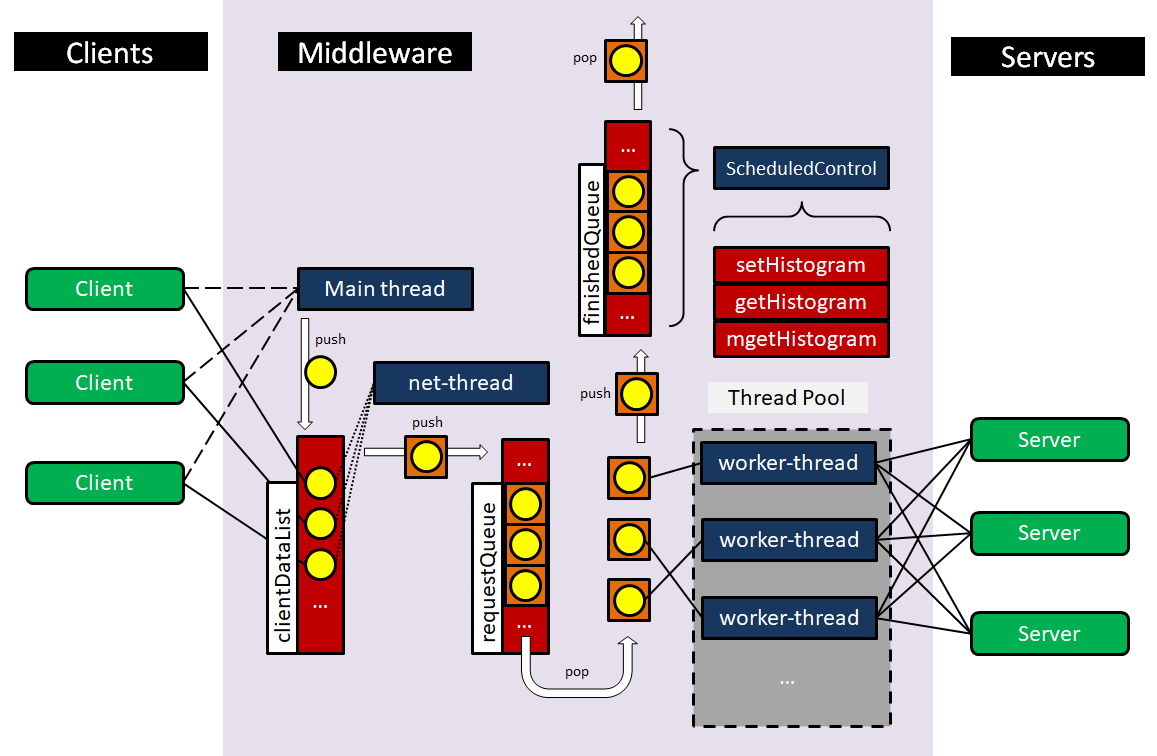
\includegraphics[width=0.8\linewidth,trim={0px 0px 0px 0px},clip]{img/system-diagram.png}
  \caption{A simplified diagram of the system showing the inner structure of the system and the interaction of its components in an informal manner. Yellow circles represent the clientData objects and the orange squares represent the requestData objects, whose instances encapsulate the ones of the former. Dark blue rectangles represent the threads in the system, of which there are always three plus the size of the worker thread pool. Red rectangles represent the shared lists and queues which form the pipeline and help aggregation of the statistics. Green rounded rectangles illustrate the external systems, namely the clients and servers. Dashed line shows the communication with the welcomingSocket and the dotted line is net-thread checking if there is any request available. Solid lines represent the main information flow from clients to servers and again back to the clients.}
  \label{fig:system-diagram}
\end{figure}

\subsubsection{Main thread} \label{sec:overview-mainthread}
Main thread of the \underline{MyMiddleware} class is responsible for setting up the working environment for the whole system. It first initializes the shared data structures that are to be used by other threads; namely, these are \underline{clientDataList} (which stores information about each one of the connected clients), \underline{requestQueue} (which is a first-in, first-out queue for queries awaiting execution) and \underline{finishedQueue} (which temporarily stores the completed requests for the aggregation of their statistics). It then creates a \underline{clientHandler} (so-called \say{net-thread}, which is responsible for handling communication with clients) and the specified number of \underline{serverHandler} threads (so-called \say{worker-threads}, which are responsible with for handling communication with the servers). Throughout this report, names clientHandler and net-thread will be used interchangeably. Same also applies for worker-threads and serverHandlers. Lastly, the main thread creates the \underline{welcomingSocket} and listens for incoming client connections in a loop. As soon as such a connection request is received, main thread creates the respective \underline{clientData} object and pushes it into the clientDataList. welcomingSocket has a backlog queue for 512 connections, so it is expected to handle at most 512 concurrent incoming connections. This size is more than we will ever need with our experiments and provided as a safety measure.
\par
clientData objects store the information relevant for communicating with the clients. They consist of the net socket, its respective reader and writer streams, an identifier number and lastly a flag that denotes if the client has already sent its request and awaiting for reply.

\subsubsection{clientHandler (net-thread)} \label{sec:ov-netthread}
The clientHandler constantly iterates over the clientDataList, waiting for new requests from clients. It employs busy waiting as it non-blockingly check each client to see if there is an available request. As soon as it receives its first query from a client, clientHandler initializes the \underline{ScheduledControl} thread, which is responsible for periodically aggregating statistics of the system. clientHandler checks for each client if it has not been waiting for a repy and data is available in its reader stream. That means that client has a new request so the clientHandler creates a new \underline{RequestData} object and pushes it into the requestQueue for it to be handled by the worker-threads. clientHandler thread does not parse or modify the requests and directly transfer them to the worker-threads.
\par At the beginning of each iteration over the clientDataList, clientHandler compares the time with the timestamp of the last received query. If it is larger than some safe threshold, that means no other requests will arrive for our working conditions, so it moves on to close the system killing all threads. Before exiting clientHandler prints the response time histograms created by the ScheduledControl thread.
\par requestData objects contain the necessary relevant information about a request so that it can be executed correctly and its statistics can be aggregated with ease. Aside from information about its respective client, it stores an identifier number, the type of the request (set, get or multi-get), which server the request is sent to (if it is a get or multi-get request), which worker-thread handled the request, how many items were requested and received (if it is a get or multi-get request) and its timestamps.
\begin{figure}[h!]
  \centering
  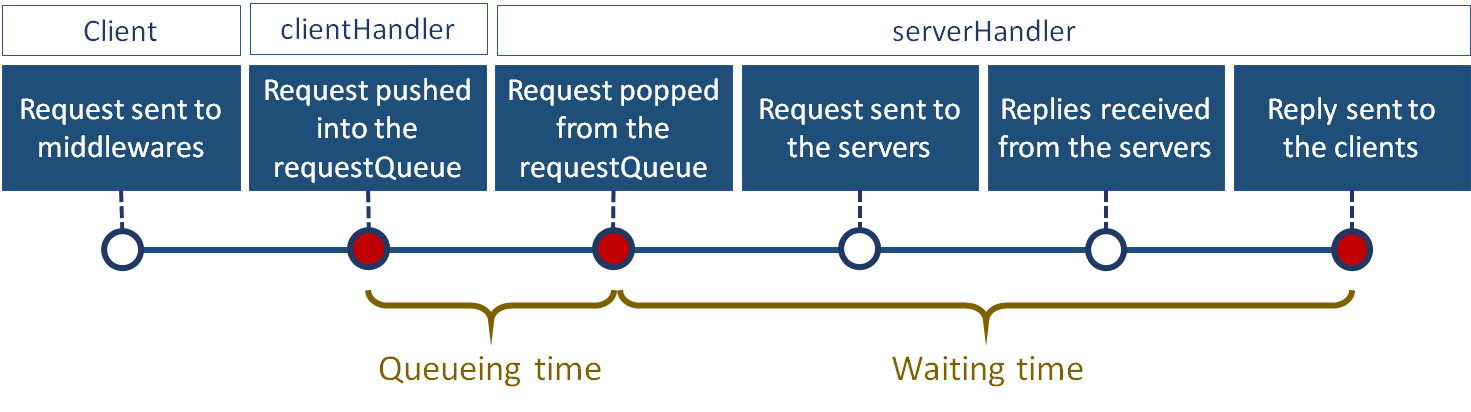
\includegraphics[width=0.8\linewidth,trim={0px 0px 0px 0px},clip]{img/timing.png}
  \caption{A diagram showing the timestamping of the requests. Line shows the lifetime of a request where the red circles denote the actions where a timestamp is collected. Names above show where the specified actions take place.}
  \label{fig:timing}
\end{figure}
\par Timestamps are all obtained in nanoseconds using Java's \texttt{System.nanoTime}. \underline{ns\_netThreadReceived} marks the time net-thread received the request from the client. \underline{ns\_workerThreadReceived} marks the time the request has exited the request queue to be handled by a worker-thread. The difference of those two timestamps give the \textbf{waiting time in the queue}. Lastly, there is \underline{ns\_workerThreadFinished} that marks the worker-thread received an answer from the servers (either successful or not) and replied to the querying client for the request. The difference of this last two timestamps (namely ns\_workerThreadFinished and ns\_workerThreadReceived) gives the \textbf{service time of the memcached servers}. The terms queueing time and waiting time in the discussions that take place in the later sections refer respectively to waiting time in the queue and the service time of the memcached servers. Figure \ref{fig:timing} illustrates where the timestamps are collected and how these times are calculated.

\subsubsection{serverHandlers (worker-threads)} \label{sec:ov-workerthread}
serverHandler threads initially set up dedicated connections to each server with their reader and writer streams. They also operate in an infinite loop, waiting for new request to take from the requestQueue in a blocking manner. It is blocking as a worker thread has no other jobs than handling requests. As soon as there is an available request in the queue the worker-thread wakes up, marks the time and unpacks the requestData structure. \textbf{Worker-threads are the ones that parse the messages}, so the certain specifics of the requests are unknown to the system until they exit the queue. After it has been handled accordingly to its type, the resulting requestData is pushed into the finishedQueue.
\begin{figure}[h]
  \centering
  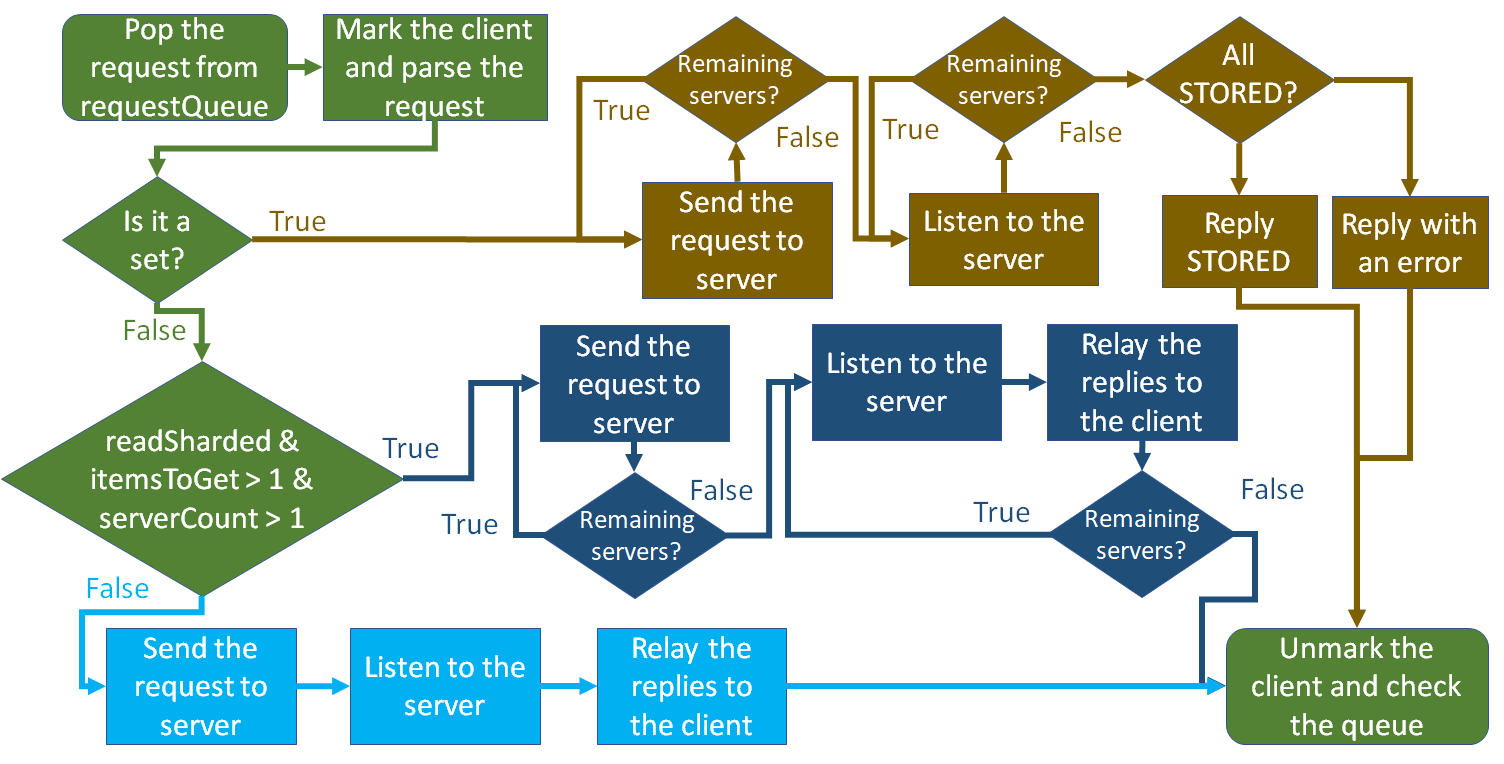
\includegraphics[width=1.0\linewidth,trim={0px 0px 0px 0px},clip]{img/flowchart.png}
  \caption{Flowchart showing one iteration of a worker thread in its infinite loop. States are color coded where the gold, light blue and dark blue states are respectively for set, get and multi-get operations. Green states denote states that are common for multiple types of operations. Each thread run its own round-robin over the available servers.}
  \label{fig:flowchart}
\end{figure}
\par If it is a set query, the request is sent to all of the servers and reported as successful to the client only if all the responses indicate so. If not, one of the error messages are relayed to the sender client. If it is a get request there are two possibilities. If it is a multi-get request in a multi-server setting with \texttt{readSharded} option provided as true, then it is sharded into smaller requests. If the query requests a single object, there is a single server or \texttt{readSharded} is provided as false, then the request will be sent to only one server. In either case, middleware employs a simple load balancing scheme through a round-robin scheduling. It iterates over all servers while sending get requests or the sharded get requests. For both set and get requests middleware first sends the requests to servers and then collect the responses. Flowchart illustrating the state flow of the system when handling different types of operations can be viewed in Figure \ref{fig:flowchart}. Middleware outputs for the later experiments confirm that the workload is indeed distributed equally to multiple servers, as seen on Figure \ref{fig:equal-load}.
%
%\begin{figure}[h]
%\centering
%\begin{subfigure}{.33\textwidth}
%  \centering
%  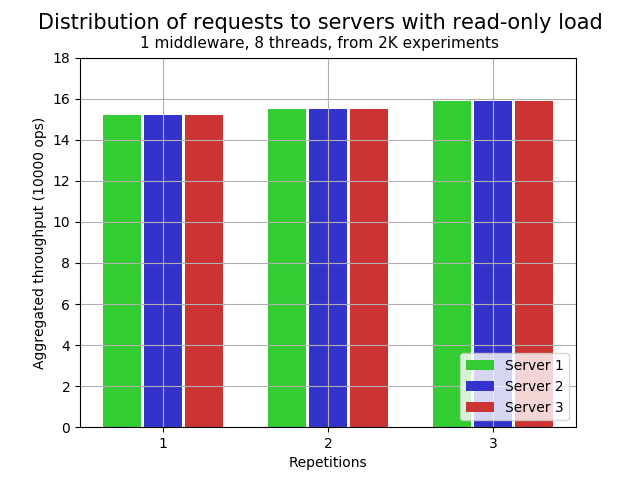
\includegraphics[width=1.0\linewidth,trim={0px 0px 0px 0px},clip]{img/plot/equal-load-read-only.png}
%  \caption{Read-only load}
%  \label{fig:equal-load-read-only}
%\end{subfigure}%
%\begin{subfigure}{.33\textwidth}
%  \centering
%  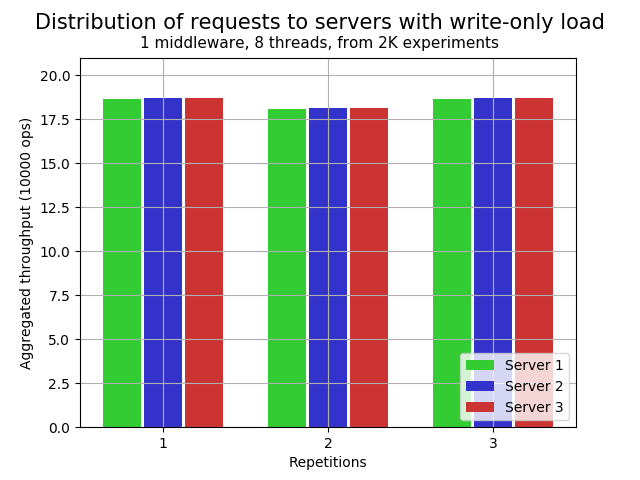
\includegraphics[width=1.0\linewidth,trim={0px 0px 0px 0px},clip]{img/plot/equal-load-write-only.png}
%  \caption{Write-only load}
%  \label{fig:equal-load-write-only}
%\end{subfigure}%
%\begin{subfigure}{.33\textwidth}
%  \centering
%  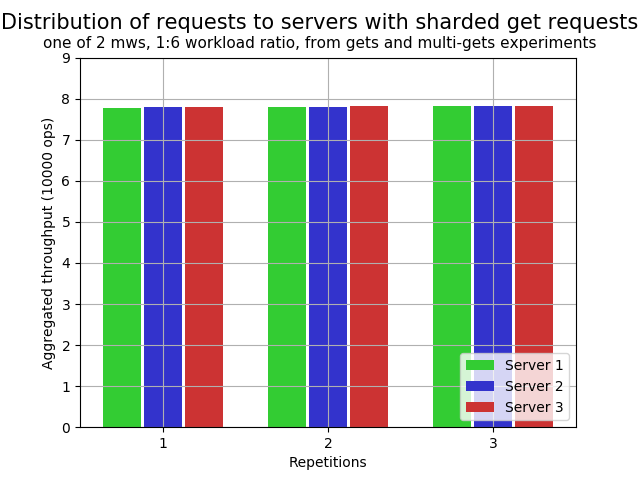
\includegraphics[width=1.0\linewidth,trim={0px 0px 0px 0px},clip]{img/plot/equal-load-sharded-get.png}
%  \caption{Sharded get requests}
%  \label{fig:equal-load-sharded-get}
%\end{subfigure}
%\caption{Distribution of the requests to three servers over three repetitions. Each of the plots illustrate a different workload condition. Results are taken from the experiments of later sections. Figures \ref{fig:equal-load-read-only} and \ref{fig:equal-load-write-only} use the results from 2K experiments \ref{sec:2k} and Figure \ref{fig:equal-load-sharded-get} use those from gets and multi gets experiments \ref{sec:gmg}}
%\label{fig:equal-load}
%\end{figure}

\begin{figure}[h]
  \centering
  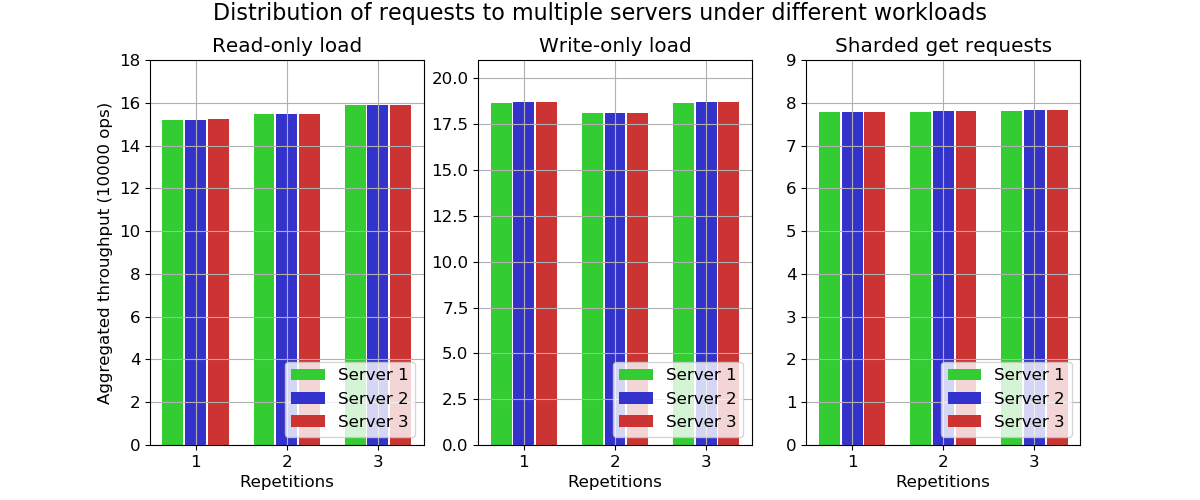
\includegraphics[width=1.0\linewidth,trim={0px 0px 0px 0px},clip]{img/plot/equal-load-all.png}
\caption{Distribution of the requests to three servers over three repetitions. Each of the plots illustrate a different workload condition. Results are taken from the experiments of later sections. First two plot use the results from 2K experiments \ref{sec:2k} and the last plot use those from gets and multi gets experiments \ref{sec:gmg}. Experiment with read-only and write-only loads inspect 1 middleware with 8 threads, whereas the sharded read experiment is plotted using aggregated results for the get requests in one of the two middlewares, on 1:6 workload ratio.}
\label{fig:equal-load}
\end{figure}

\subsubsection{ScheduledControl} \label{sec:ov-scheduledcontrol}
ScheduledControl is started by the net-thread as it receives its first request. It periodically wakes up, aggregates the statistics over the most recent requests, then sleeps again. It goes over the entries in finishedQueue in its each run, collecting type-specific statistics. \textbf{For all our experiments, the aggregation period is set as 1 second}.
\par The thread aggregates the number of requests, queue waiting times and server waiting times separately for set, get and multi-get requests. For multi-get and get times, overall miss-rate is also aggregated together. Miss-rates are calculated over the total number of distinct get requests, breaking apart the multi-gets. For example, for two multi-gets with 5 keys if one item in one multi-get is a cache miss, the miss-rate is reported as 10\%, not as 50\%.
\par ScheduledControl also keeps track of the distribution of the response times for different types of requests by constructing a separate histogram for each type of request, namely sets, gets and multi-gets. While going over the list of requests the ScheduledControl assigns each of the requests to the appropriate histogram bin with respect to its response time and type. Lastly, length of the requestQueue is saved in each run of the ScheduledControl.

\subsection{Methodology} \label{sec:ov-methodology}
\par Three repetitions were seem to be sufficient all the experiments as both our middleware and the external systems it communicated had shown performances that stayed fairly stable under repetitions. Similarly, trimming five seconds of warm-up and cool-down periods, respectively at the beginning and the end of experiments, was found as sufficient through the initial exploratory experiments performed. Clients can lag behind around at most one second per a three repetition run, but it is still negligible with the times cut for warm-up and cool-down periods. Baseline without middleware experiments (Section \ref{sec:csb}) were run for 100 seconds per each iteration, yielding a one and a half minute period after cutting the warm-up and cool-down times. Experiments involving middleware (Sections \ref{sec:mwb}, \ref{sec:tpfw}, \ref{sec:gmg} and \ref{sec:2k} consists of three repetitions of 70-second runs yielding a 60 second stable period for aggregation.
\par iPerf3 \cite{iperf} is used to measure the maximum achievable bandwith in between different machines in our environment. The results can be seen in Table \ref{tab:iperf3-bandwidth}. For each machine in every experiment, we collect data through dstat \cite{dstat}. dstat is run in its default mode, so it collects statistics cpu, disk, network, paging and system  statistics. It collects data every second after an initial delay of one second — similar to the ScheduledControl in our middleware.
\begin{table}[h]
\centering
\resizebox{\textwidth}{!}{
\begin{tabular}{|c|c|c|c|}
\hline 
Machine & Bandwidth (Mbps) & Bandwidth (MB/s) & Effective bandwidth* (MB/s) \\ 
\hline 
Client & 200 & 25 & $\sim 24$ \\ 
\hline 
Middleware & 800 & 100 & $\sim 96$ \\ 
\hline 
Server & 100 & 12.5 & $\sim 12$ \\ 
\hline 
\end{tabular}}
{*: for read-only and write-only workloads}
\caption{Maximum achievable bandwidth values for all machines, obtained using iperf3. So-called ``effective bandwidth'' is the maximum bandwidth a machine can utilize only with the set queries or get replies. It is an informal measure that comes as useful while analyzing read-only and write-only workloads in later sections.} \label{tab:iperf3-bandwidth}
\end{table}
\par We illustrate the dispersion over different repetitions of individual experiments through standard variance. For every plot, error bars indicate a range of one standard variance calculated over the repetitions. At times such error bars may not be visible to the reader, indicating a fairly robust experimental setup. Most of the plots have their x-axis as the number of clients. It is the effective number of different clients and is simply calculated by multiplying four numbers: number of virtual clients per thread, number of threads per memtier instance, number of memtier instances per virtual machine and the number of client machines. Using the abbreviations in Table \ref{tab:param-abbrs} the formula could be written as $numClients = vcli \times tcli \times icli \times ncli$. The term latency is used interchangeably with the term response time. Plots specify the source of measurements as middlewares or clients in their subtitles, so it is easy to find for a plot whose perspective it reflects. It should be also noted here that for each separate experiment where the number of virtual clients are varied, we always make sure that at least 6 different values for virtual clients per client thread are explored.
\par For every experiment, interactive law is verified by both calculating the throughput from the response times and vice versa. As it would approximately double all the plots we provide here to show that the interactive law indeed holds for all the experiments, we only provide the illustration of this guarantee in Section \ref{sec:csb}. Figures \ref{fig:csb1-wo-law}, \ref{fig:csb1-ro-law}, \ref{fig:csb2-wo-law} and \ref{fig:csb2-ro-law} show the actual and predicted values coincide perfectly. Reader should feel free to run the provided scripts for other experiments and see the interactive law in action in other experiments as well.
\\
\par In  experiments involving the get operations the servers are always populated beforehand so miss rates are either realistic and negligible. Server population is always done in the same manner: first 99\% of the keys that are to be used in experiments were set by the sequential load option of the memtier. Therefore, for all the get requests we expect similar miss rates which are around 1\%. Some actual miss rates, from the baseline with middleware experiments, can be viewed in Section \ref{sec:mwb-summary}.


\section{Baseline without Middleware} \label{sec:csb}
In this section, we examine the characteristics of the clients and servers before the introduction of the middleware to the environment. For all different configurations of different experiments we show that the interactive law holds true by calculating the throughput values from the response times and vice versa. Values predicted through the interactive law are always illustrated alongside the actual values obtained by the memtier outputs.

\subsection{One Server} \label{sec:csb1}
First setting contains three memtier clients connecting to one memcached server. Each of the client machines has one memtier instance with two client threads running in them. We vary the number of virtual clients and the type of workload (write-only and read-only) and observe the change in the performance of the system.

\begin{figure}[h]
\centering
\begin{subfigure}{.5\textwidth}
  \centering
  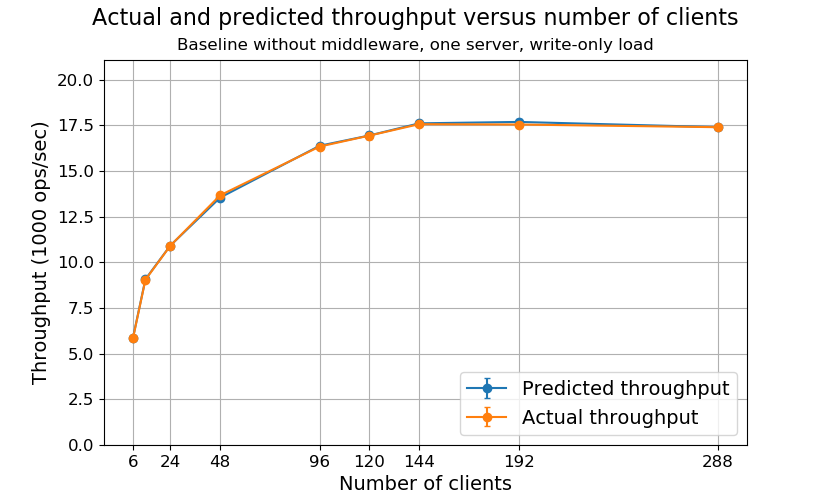
\includegraphics[width=1.0\linewidth,trim={20px 0px 35px 0px},clip]{img/plot/csb1-wo-law_tpt.png}
  \caption{Write-only throughput}
  \label{fig:csb1-wo-law_tpt}
\end{subfigure}%
\begin{subfigure}{.5\textwidth}
  \centering
  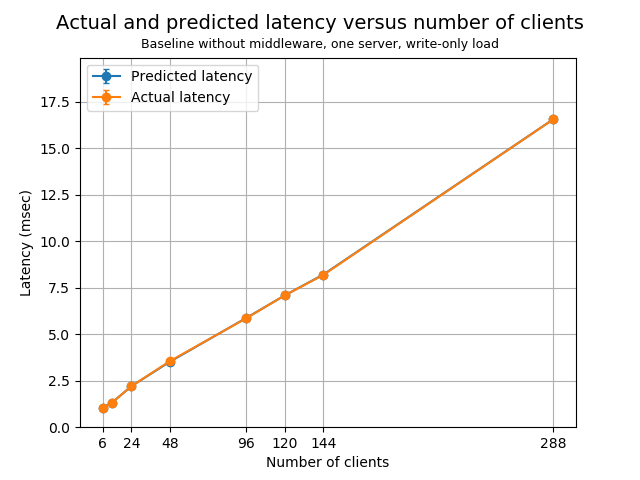
\includegraphics[width=1.0\linewidth,trim={20px 0px 40px 0px},clip]{img/plot/csb1-wo-law_lat.png}
  \caption{Write-only latency}
  \label{fig:csb1-wo-law_lat}
\end{subfigure}
\caption{Throughput and latency values for the write-only workload for baseline without middleware, for one server case.}
\label{fig:csb1-wo-law}
\end{figure}

\begin{figure}[h]
\centering
\begin{subfigure}{.5\textwidth}
  \centering
  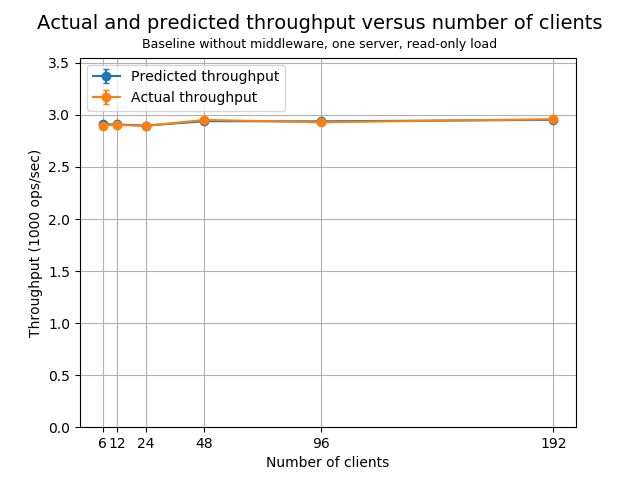
\includegraphics[width=1.0\linewidth,trim={20px 0px 35px 0px},clip]{img/plot/csb1-ro-law_tpt.png}
  \caption{Read-only throughput}
  \label{fig:csb1-ro-law_tpt}
\end{subfigure}%
\begin{subfigure}{.5\textwidth}
  \centering
  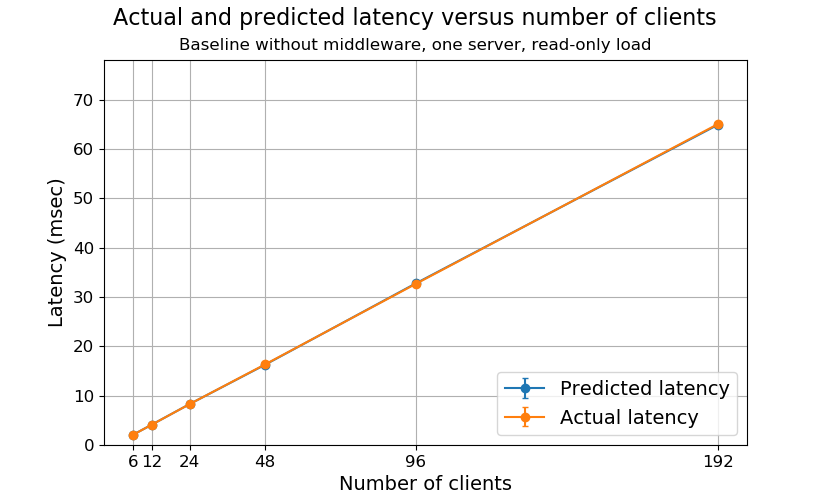
\includegraphics[width=1.0\linewidth,trim={20px 0px 40px 0px},clip]{img/plot/csb1-ro-law_lat.png}
  \caption{Read-only latency}
  \label{fig:csb1-ro-law_lat}
\end{subfigure}
\caption{Throughput and latency values for the read-only workload for baseline without middleware experiment with one server case.}
\label{fig:csb1-ro-law}
\end{figure}

\subsubsection{Explanation} \label{sec:csb1-exp}
We see the results for the one server configuration in Figures \ref{fig:csb1-wo-law} and \ref{fig:csb1-ro-law}. Plots show that the interactive law holds true for both experiments.

\par For the write-only part, we can observe the system starts as undersaturated and begins to saturate after 96 clients. Throughput increases steadily until the saturation point, as additional clients are connected to the system. Afterwards we can observe only marginal increases in the throughput until 144 clients, where the system reaches its maximum throughput of $17556.5$ requests in average. After 144 clients, the system acts as undersaturated as any additional clients hinder performance, even lowering the throughput values. We see a similar trend in the response time plot as it is slightly curved until around the saturation point but linear afterwards. After the saturation point, the system cannot handle any more requests and the average response time increases linearly with respect to number of clients while there is no increase in throughput values as the system is already at full capacity. We state 96 clients is the saturation point as it is where the performance yields starts to get more unnoticeable. Going from 96 to 120 or 120 to 144 clients only account for increases around 3\% whereas response times continue to increase approximately 20\% and 15\% respectively.
\par The reason behind this saturation is meeting the network bandwidth capacity. dstat files show that each client can send at most 24MB per second on average. Looking at the iperf results (Table \ref{tab:iperf3-bandwidth}) we can see that client to server communication is limited by 24MB per second for different configurations. As we send 4096B data that means we can send $\sim 6000$ requests per machine, $\sim 18000$ requests in total, and this corroborates our results.

\par In the read-only part, we see that the system begins operating already in the saturated region for the minimum number of clients we can achieve, which is 6. We conclude this as we cannot observe any noticeable change in throughput when we vary the number of clients and the response time is approximately a linear function of the number of clients everywhere. Although we can see the absolute maximum of the throughput plot is at 32 clients, it is clear that the system becomes highly inefficient with the addition of each additional client to the system after 6 clients. Only increases in the throughput are quite marginal whereas response times double when we double the number of clients in the system.
\par Again, dstat and iperf together confirm our assertions and indicates the reason for the saturation. iperf states the server to client connection is limited by 12MB per second (Table \ref{tab:iperf3-bandwidth}) and it is what we observe in our server for varying number of clients through all repetitions. This implies the server can reply to at most $\sim 3000$ requests per second and it is in line with our results.

\subsection{Two Servers} \label{sec:csb2}
This configuration deals with one client machine sending requests to two servers. This time the client machine has two instances of memtier running (each connected to a different server) with one client thread per instance. We again change the workload (write-only and read-only) and change the total number of clients by varying the virtual number of clients and observe the changes in the performance.

\begin{figure}[h]
\centering
\begin{subfigure}{.5\textwidth}
  \centering
  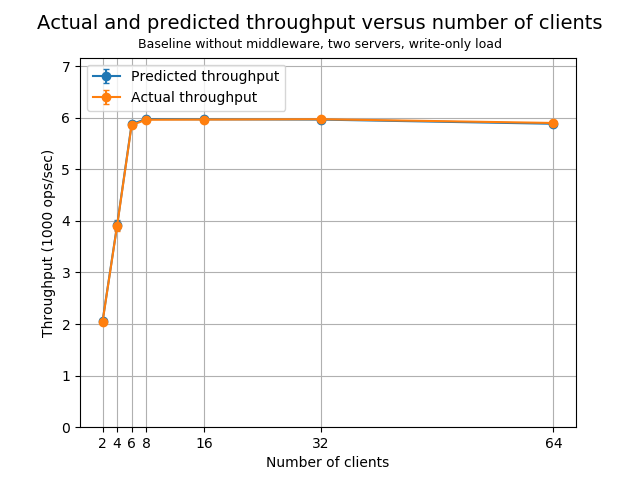
\includegraphics[width=1.0\linewidth,trim={20px 0px 35px 0px},clip]{img/plot/csb2-wo-law_tpt.png}
  \caption{Write-only throughput}
  \label{fig:csb2-wo-law_tpt}
\end{subfigure}%
\begin{subfigure}{.5\textwidth}
  \centering
  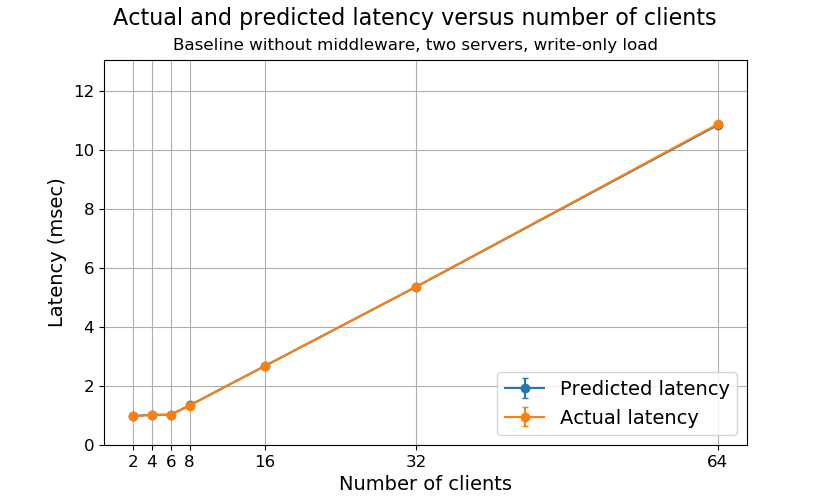
\includegraphics[width=1.0\linewidth,trim={20px 0px 40px 0px},clip]{img/plot/csb2-wo-law_lat.png}
  \caption{Write-only latency}
  \label{fig:csb2-wo-law_lat}
\end{subfigure}
\caption{Throughput and latency values for the write-only workload for baseline without middleware experiment with two servers.}
\label{fig:csb2-wo-law}
\end{figure}

\begin{figure}[h]
\centering
\begin{subfigure}{.5\textwidth}
  \centering
  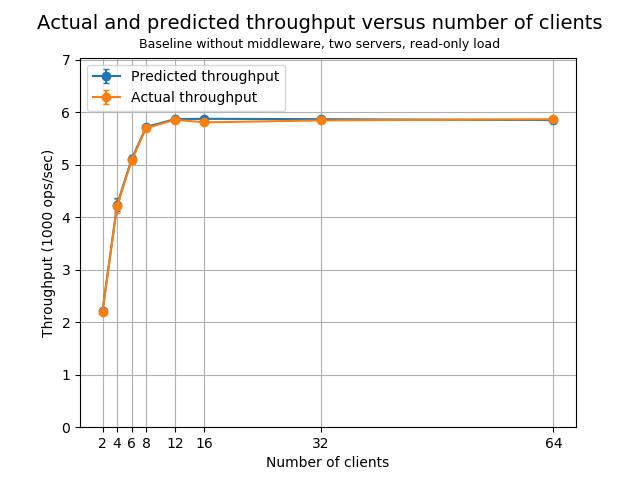
\includegraphics[width=1.0\linewidth,trim={20px 0px 35px 0px},clip]{img/plot/csb2-ro-law_tpt.png}
  \caption{Read-only throughput}
  \label{fig:csb2-ro-law_tpt}
\end{subfigure}%
\begin{subfigure}{.5\textwidth}
  \centering
  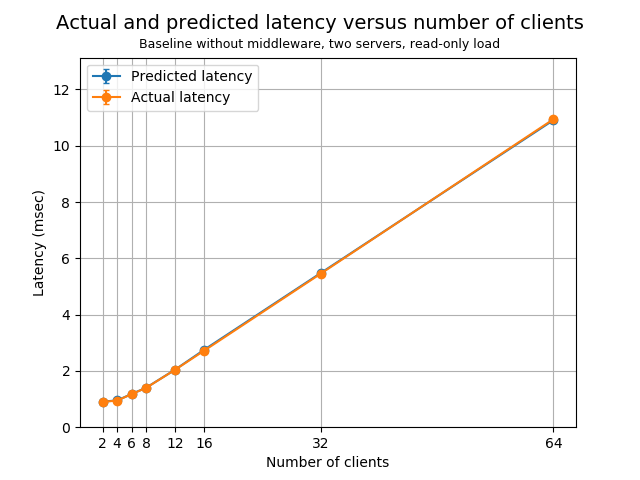
\includegraphics[width=1.0\linewidth,trim={20px 0px 40px 0px},clip]{img/plot/csb2-ro-law_lat.png}
  \caption{Read-only latency}
  \label{fig:csb2-ro-law_lat}
\end{subfigure}
\caption{Throughput and latency values for the read-only workload for baseline without middleware experiment with two servers.}
\label{fig:csb2-ro-law}
\end{figure}

\subsubsection{Explanation} \label{sec:csb2-exp}
Results are illustrated in Figures \ref{fig:csb2-wo-law} and \ref{fig:csb2-ro-law}. Unlike the first part, we obtain similar trends in plots for both the read-only and the write-only case.
For the write-only case, we see the system beings as undersaturated, saturates around 6 clients and reaches its maximum throughput at 8 clients where the throughput plot seems to level off. Figure \ref{fig:csb2-wo-law_lat} corroborates our comments as the response times stay stable up to 6 clients, start to increase until 8 clients and become completely linear after it crosses 8 clients.
\par Similarly, for the read-only case, we conclude the system begins as undersaturated and saturates around 8 clients. Then the system reaches its maximum throughput at 12 clients and again acts as saturated afterwards. We argue that 8 clients is the saturation point as moving from 6 to 8 clients result in comparable changes in both throughput and response times (12\% and 19\%), moving from 8 to 12 clients bring only marginal increases with respect to throughput (2.7\%) but considerable increases in average response times (46\%). We can also see that the response times are quite low and almost stable until 8 clients. Similarly to what we have seen before response time plot becomes linear as we move past the saturation point.
\par The main reason behind the saturation can be found in the network bandwidth limitations for both cases. Although intuitively, the write-only and read-only cases have their bottlenecks in different parts of the network pipeline. Situation is quite similar to the earlier results in Section \ref{sec:csb1}. For the write-only case, dstat outputs for the saturated configurations show that the client sends at most 24MB per second to servers, which is its limit confirmed by iperf statistics (Table \ref{tab:iperf3-bandwidth}). This corresponds to a total of $\sim 6000$ requests distributed to two servers, corroborating our results. We also know through iperf that a server can send at most 12MB per second (Table \ref{tab:iperf3-bandwidth}) and and we see the same numbers in our dstat files for the read-only part. This equals to 24MB per second received by clients, again amounting to a total of $\sim 6000$ requests, this time as a result of another limiting factor.

\subsection{Summary} \label{sec:csb-summary}
Here, we comparatively analyse the different results for the previously discussed set of experiments. The results are explained in more detail in Sections \ref{sec:csb1-exp} and \ref{sec:csb2-exp}, so we will not be going into the specifics of each experiment here.
\begin{table}[h]
\small
\centering
{Maximum throughput of different VMs.}
\begin{tabular}{|l|p{2.1cm}|p{2.2cm}|p{6cm}|}
\hline 	                      & Read-only workload & Write-only workload & Configuration gives max. throughput \\ 
\hline One memcached server & $2897.9 \pm 16.4$ & $17556.5 \pm 50.1$ & read-only: 6, write-only: 144 clients \\ 
\hline One load generating VM & $5856.1 \pm 12.6$ & $5960.9 \pm 3.2$   & read-only: 12, write-only: 8 clients \\ 
\hline 
\end{tabular}
\caption{Summary of baseline without middleware experiments.} \label{tab:csb-summary}
\end{table}
\par Table \ref{tab:csb-summary} reports the maximum throughput obtained in both experiments and the configurations that allow such maxima. For both experiments under either read-only or write-only workload conditions, we have concluded that the bottleneck of the system is always the network bandwidth. Intuitively enough, write-only requests have large queries and small responses as they send the data to be stored and only return with a confirmation or an error message. The situation is reversed for the read-only workload as get requests merely contain the keys but their replies carry the data itself (as we get a hit rather than a miss almost everywhere). Therefore, it is in line with our expectations that the throughput values for the experiments with write-only workload are limited by the client to server bandwidth and similarly, throughput values for the read-only counterparts are limited by the server to client bandwidth.
\par These arguments are clearly evidenced by our results in Table \ref{tab:csb-summary}. Maximum read-only throughput doubles as we introduce another server to our one server setting. Similarly for the write-only workload, by going from three load generating machines to a one client setting we can see expect the maximum throughput to become one third of what it was before.
\\
\par As a side note, we observe only the write-only workload with three client machines resulting a appreciable percentage of CPU usage in servers, in the saturated region. Aside from this specific case not one server or client experience any high CPU utilization, idle times are consistently above $90\%$.
\par It is also worth noting that for the read-only workload in one server setting (Section \ref{sec:csb1-exp}) we state the system is already saturated with the presence of 6 clients, even though we do not have any information regarding the fewer number of clients. It is the outcome of a comparison with the read-only experiments with two servers and one client, as we notice that with 6 clients on client machine can help achieve a throughput around 2000 requests. Keeping in mind that the server performance is not a bottleneck anywhere in these experiments we can expect that three clients in one server hypothetically achieving a throughput of 6000 requests whereas the actual value is only the half of it. Then we conclude that system theoretically saturates even earlier, whose effective number of clients we cannot observe with our experimental design.

\section{Baseline with Middleware} \label{sec:mwb}
In this section, we observe the changes in the overall system when the middleware is introduced to the environment, as well as we discuss the characteristics of the middleware that we can observe in the scope of this set of experiments. Interactive law for every experiment is verified using the measurements on clients. More discussion on interactive law can be found at the end of Section \ref{sec:mwb-summary}.

\subsection{One Middleware} \label{sec:mwb1}
First experiment for this section is conducted on three client machines connected to one middleware, which in turn connected to one server. Apart from experimenting with two workloads (read-only and write-only) and varying the number of virtual clients we also change the number of worker threads in the middleware.
\begin{figure}[h!]
\centering
\begin{subfigure}{.5\textwidth}
  \centering
  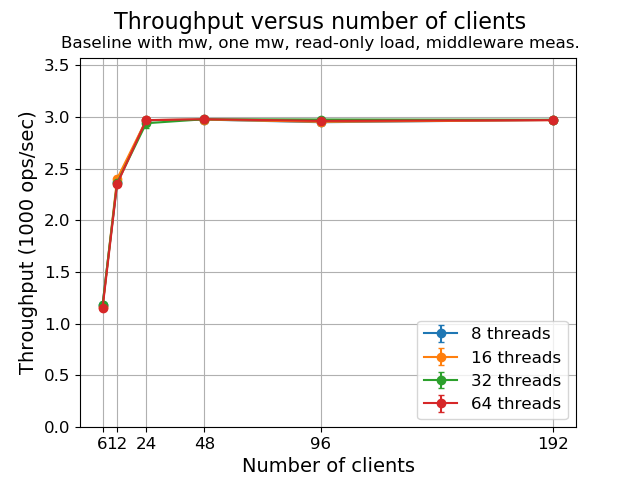
\includegraphics[width=1.0\linewidth,trim={5px 0px 20px 0px},clip]{img/plot/mwb1-ro-tp_mw.png}
  \caption{Read-only throughput}
  \label{fig:mwb1-ro-tp_mw}
\end{subfigure}%
\begin{subfigure}{.5\textwidth}
  \centering
  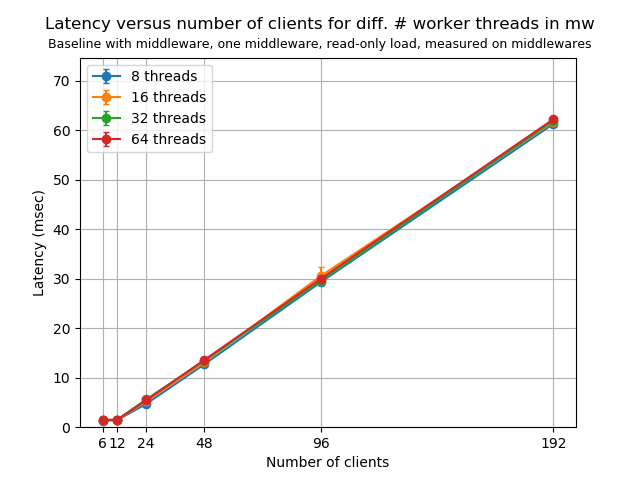
\includegraphics[width=1.0\linewidth,trim={5px 0px 20px 0px},clip]{img/plot/mwb1-ro-lat_mw.png}
  \caption{Read-only latency}
  \label{fig:mwb1-ro-lat_mw}
\end{subfigure}
\caption{Throughput and latency values for the read-only workload for baseline with middleware experiment with one middleware.}
\label{fig:mwb1-ro_mw}
\end{figure}
\begin{figure}[h!]
\centering
\begin{subfigure}{.5\textwidth}
  \centering
  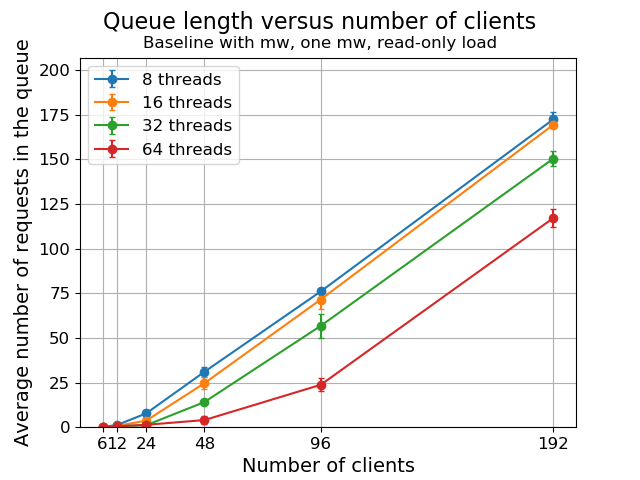
\includegraphics[width=1.0\linewidth,trim={5px 0px 20px 0px},clip]{img/plot/mwb1-ro-qlen_mw.png}
  \caption{Avg. queue length}
  \label{fig:mwb1-ro-qlen_mw}
\end{subfigure}%
\begin{subfigure}{.5\textwidth}
  \centering
  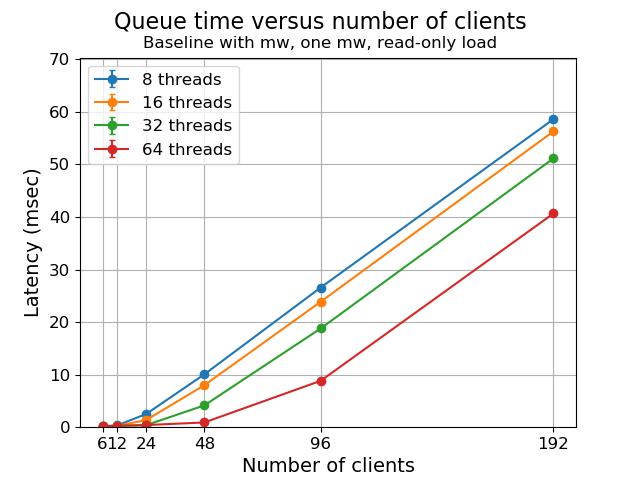
\includegraphics[width=1.0\linewidth,trim={5px 0px 20px 0px},clip]{img/plot/mwb1-ro-qtime_mw.png}
  \caption{Avg. queue time}
  \label{fig:mwb1-ro-qtime_mw}
\end{subfigure}
\caption{Average queue lengths and queue times for the read-only workload for baseline with middleware experiment with one middleware.}
\label{fig:mwb1-ro-qstats}
\end{figure}

\subsubsection{Explanation} \label{sec:mwb1-exp}
\begin{figure}[h]
\centering
\begin{subfigure}{.5\textwidth}
  \centering
  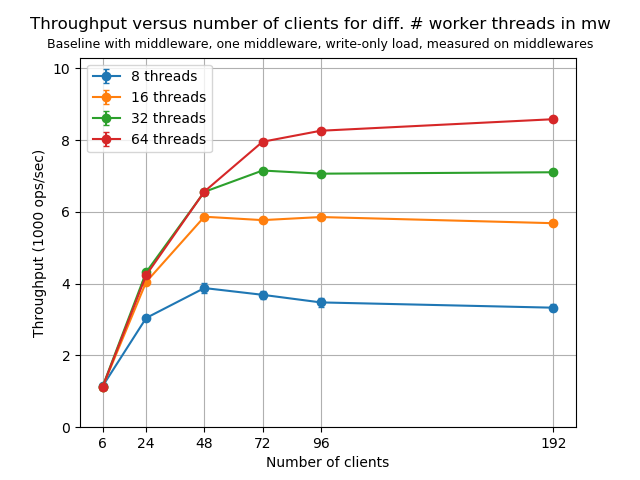
\includegraphics[width=1.0\linewidth,trim={5px 0px 20px 0px},clip]{img/plot/mwb1-wo-tp_mw.png}
  \caption{Write-only throughput}
  \label{fig:mwb1-wo-tp_mw}
\end{subfigure}%
\begin{subfigure}{.5\textwidth}
  \centering
  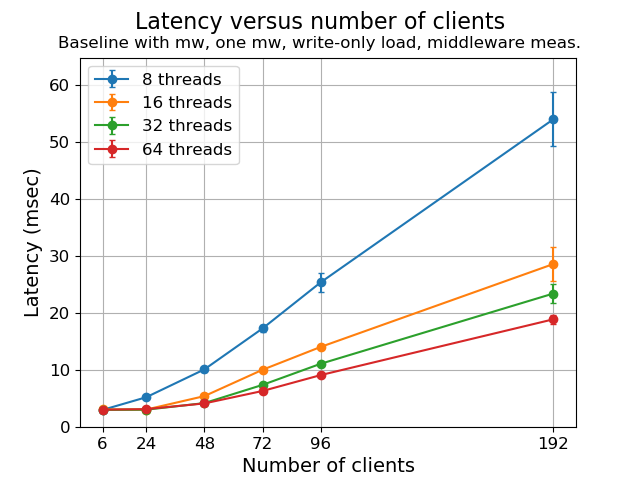
\includegraphics[width=1.0\linewidth,trim={5px 0px 20px 0px},clip]{img/plot/mwb1-wo-lat_mw.png}
  \caption{Write-only latency}
  \label{fig:mwb1-wo-lat_mw}
\end{subfigure}
\caption{Throughput and latency values for the write-only workload for baseline with middleware experiment with one middleware.}
\label{fig:mwb1-wo_mw}
\end{figure}

\begin{figure}[h]
\centering
\begin{subfigure}{.5\textwidth}
  \centering
  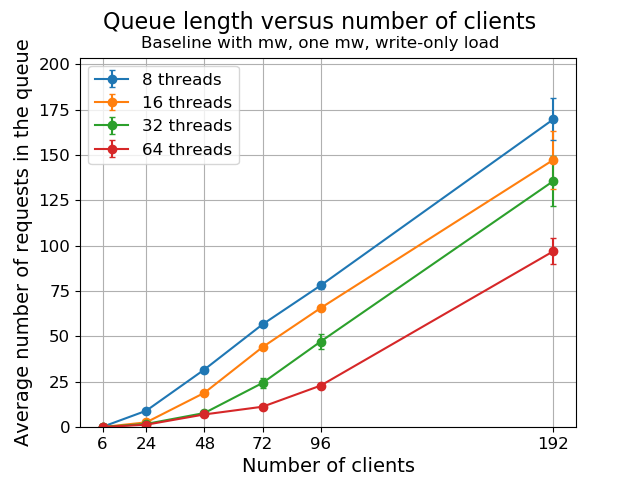
\includegraphics[width=1.0\linewidth,trim={0px 0px 0px 0px},clip]{img/plot/mwb1-wo-qlen_mw.png}
  \caption{Avg. queue length}
  \label{fig:mwb1-wo-qlen_mw}
\end{subfigure}%
\begin{subfigure}{.5\textwidth}
  \centering
  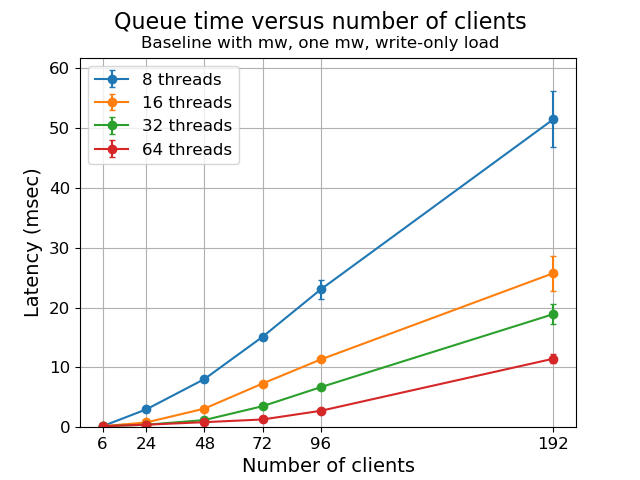
\includegraphics[width=1.0\linewidth,trim={0px 0px 0px 0px},clip]{img/plot/mwb1-wo-qtime_mw.png}
  \caption{Avg. queue time}
  \label{fig:mwb1-wo-qtime_mw}
\end{subfigure}
\caption{Average queue lengths, queue times and waiting times for the write-only workload for baseline with middleware experiment with one middleware.}
\label{fig:mwb1-wo-qstats}
\end{figure}
Plots in Figures \ref{fig:mwb1-ro_mw} and \ref{fig:mwb1-wo_mw} illustrate the throughput and response time measured on the middleware, respectively for read-only and write-only loads. With the read-only load, we observe a trend quite similar to the read-only results in baselines without middleware. Until we reach around 24 clients we can observe quite an increase in the throughput which is only accompanied by relatively smaller increases in the response time, regardless of the size of the thread pool in middleware. Afterwards, the trend is again the same for different number of threads: an increase in the number of clients results in a linear increase in the response times and does not change the average throughput obtained. Therefore, we state that the system saturates and reaches its maximum throughput when there are around 24 clients in the system, regardless of the size of the worker thread pool in the middleware.
\par The reason behind this saturation is familiar to us from the previous sections: server to middleware connection is limited by a bandwidth of 12MB per second (Table \ref{tab:iperf3-bandwidth}), so the server cannot send more replies because of the network limitations. This saturation happens so early in the system that we do not get to observe the effects of different threads in middleware. In other words, the middleware works efficiently even with 8 worker threads until the system saturates, so any number of worker threads could hypothetically handle more work if the server could be able respond more clients. It should also be noted that we cannot observe any network-wise limitations on top of the server-side send bottleneck and the CPU usage is fairly low for all the machines in the system ($80\%$ idle time at worst), as per dstat and iperf.
\par Figure \ref{fig:mwb1-ro-qlen_mw} illustrates the average queue lengths for various configurations. We can observe the queue lengths (and correspondingly queueing times) are being insignificant for all configurations until around 24 clients where we observe the saturation. As the saturated system is network bound for this workload, the server can only reply a portion of the requests while the other worker threads wait to send their requests. As seen in Figure \ref{fig:mwb1-ro-qtime_mw}, a greater number of threads mean that requests spend less amount of time in the queue. However, from Figure \ref{fig:mwb1-wo-lat_mw}, we know that each configuration has the same average response time, meaning even a request exits the queue early it should still wait for the server to be available. Even so, greater number of threads mean a higher contention for the server usage. As the number of worker threads change the times spent in queue and waiting for the server also changes while the bottleneck stays the same. Lastly, we can see by comparing the values in Figures \ref{fig:mwb1-ro-qlen_mw} and \ref{fig:mwb1-ro-qtime_mw} that the queue times and the queue lengths have an approximately linear correlation as expected. The reason behind such relation is that as the system is network bound it is not the middleware but the server side that affects the queue times in the saturated region so changing the number of worker threads does not make a difference.
\\
\par In the write-only case, we can observe a trend which is completely different from the read-only case, as the network is no longer our bottleneck. The trend until reaching 24 clients is similar with the read-only case as differences in the number of worker threads do not correspond to a difference in terms of the performance of the system, except 8 thread configuration which saturates around 24 clients. This is because the system is under-saturated for 16, 32 and 64 threads so we can expect their throughput and response time statistics to go hand in hand as the number of worker threads do not result in a noticeable difference in these metrics under light workload conditions. As we introduce more and more clients to the system we observe more divergence with respect to performance for different number of threads in the middleware.
\par We can see that there are saturation points with different values in both axes for different worker thread configurations. For the parameters explored, we say the 8, 16, 32 and 64 thread configurations have their saturation points respectively around 24, 48, 48 and 72 clients in total. Due to the limitations of the experiment, the number of clients were not explored in depth for us to pinpoint exact saturation points for all worker thread configurations. We believe a comparably more fine-grained study might show slightly different saturation points.
\par This time, the comparison of queue lengths and queue times (Figures \ref{fig:mwb1-wo-qlen_mw} and \ref{fig:mwb1-wo-qtime_mw}, respectively) yield a different interpretation. We can clearly see that, for the same queue lengths, different number of worker threads result in different slopes for the queue times, i.e., queue length to queue time ratios increase with the number of worker threads. What that means is that as the size of the thread pool increases, the system could process a longer queue for the same queueing times in average, since there will be more worker threads available to handle the requests.
\par After interpreting all the relevant plots we can conclude that for the write-only workload the middleware is the bottleneck of the system. dstat measurements are also cross-checked and we do not report any exceptional usage in network or CPU for the write-only configurations. We say that the number of worker threads is the limiting parameter for our experiments for the write-only load and more worker threads mean better system performances. Moreover, if we were to compare the results obtained here to the ones we have discussed in Section \ref{sec:csb1}, we could see that we cannot achieve the levels of throughput reached without middleware, as the middleware acts as a bottleneck between the clients and the server for the parameters we explored. Although the middleware introduces overhead in the system especially with bookkeeping and additional network delays, we believe the difference between middleware and client performances would diminish more with additional worker threads in the middleware.

\subsection{Two Middlewares} \label{sec:mwb2}
Second experiment for this section again has an environment with three clients and one server, but two middlewares instead of one. Again, we vary the workloads, number of clients and number of worker threads in the middleware and discuss the results.


\begin{figure}[h]
\centering
\begin{subfigure}{.5\textwidth}
  \centering
  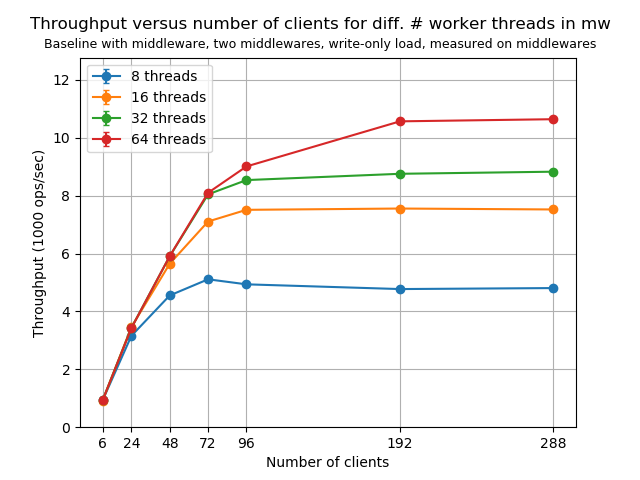
\includegraphics[width=1.0\linewidth,trim={5px 0px 20px 0px},clip]{img/plot/mwb2-wo-tp_mw.png}
  \caption{Write-only throughput}
  \label{fig:mwb2-wo-tp_mw}
\end{subfigure}%
\begin{subfigure}{.5\textwidth}
  \centering
  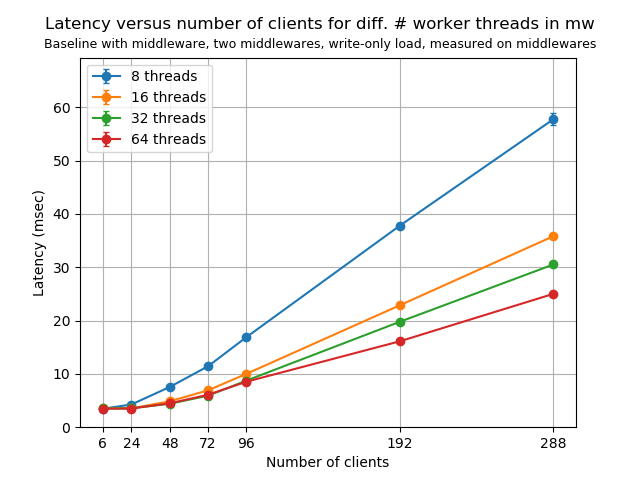
\includegraphics[width=1.0\linewidth,trim={5px 0px 20px 0px},clip]{img/plot/mwb2-wo-lat_mw}
  \caption{Write-only latency}
  \label{fig:mwb2-wo-lat_mw}
\end{subfigure}
\caption{Throughput and latency values for the write-only workload for baseline with middleware experiment with two middlewares.}
\label{fig:mwb2-wo_mw}
\end{figure}

\begin{figure}[h]
\centering
\begin{subfigure}{.5\textwidth}
  \centering
  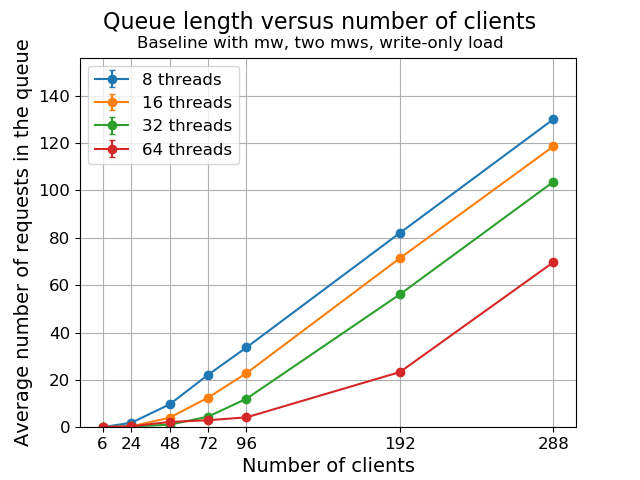
\includegraphics[width=1.0\linewidth,trim={0px 0px 0px 0px},clip]{img/plot/mwb2-wo-qlen_mw.png}
  \caption{Avg. queue length}
  \label{fig:mwb2-wo-qlen_mw}
\end{subfigure}%
\begin{subfigure}{.5\textwidth}
  \centering
  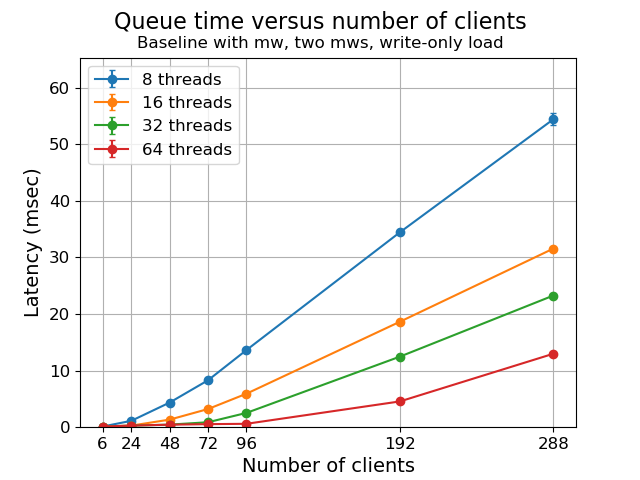
\includegraphics[width=1.0\linewidth,trim={0px 0px 0px 0px},clip]{img/plot/mwb2-wo-qtime_mw.png}
  \caption{Avg. queue time}
  \label{fig:mwb2-wo-qtime_mw}
\end{subfigure}
\caption{Average queue lengths and queue times for the write-only workload for baseline with middleware experiment with two middlewares.}
\label{fig:mwb2-wo-qstats}
\end{figure}

\begin{figure}[h]
\centering
\begin{subfigure}{.5\textwidth}
  \centering
  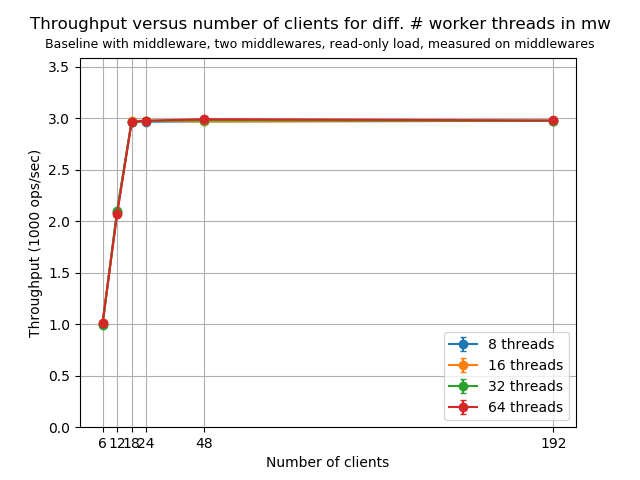
\includegraphics[width=1.0\linewidth,trim={5px 0px 20px 0px},clip]{img/plot/mwb2-ro-tp_mw.png}
  \caption{Read-only throughput}
  \label{fig:mwb2-ro-tp_mw}
\end{subfigure}%
\begin{subfigure}{.5\textwidth}
  \centering
  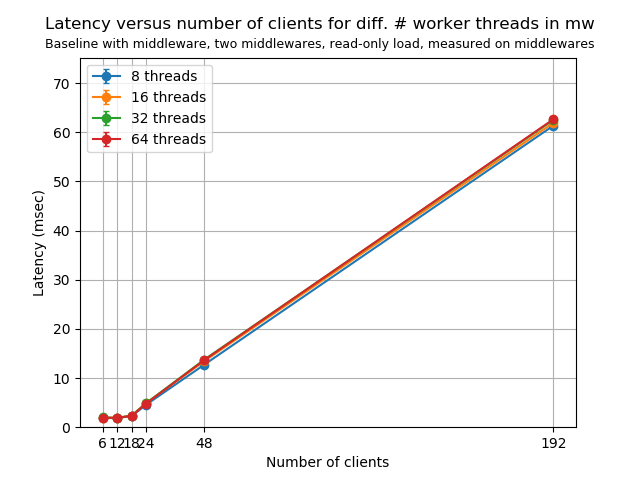
\includegraphics[width=1.0\linewidth,trim={5px 0px 20px 0px},clip]{img/plot/mwb2-ro-lat_mw}
  \caption{Read-only latency}
  \label{fig:mwb2-ro-lat_mw}
\end{subfigure}
\caption{Throughput and latency values for the read-only workload for baseline with middleware experiment with two middlewares.}
\label{fig:mwb2-ro_mw}
\end{figure}

\begin{figure}[h]
\centering
\begin{subfigure}{.5\textwidth}
  \centering
  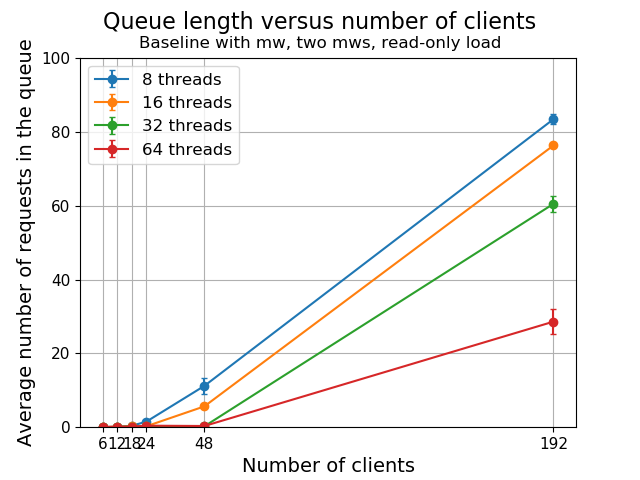
\includegraphics[width=1.0\linewidth,trim={5px 0px 20px 0px},clip]{img/plot/mwb2-ro-qlen_mw.png}
  \caption{Avg. queue length}
  \label{fig:mwb2-ro-qlen_mw}
\end{subfigure}%
\begin{subfigure}{.5\textwidth}
  \centering
  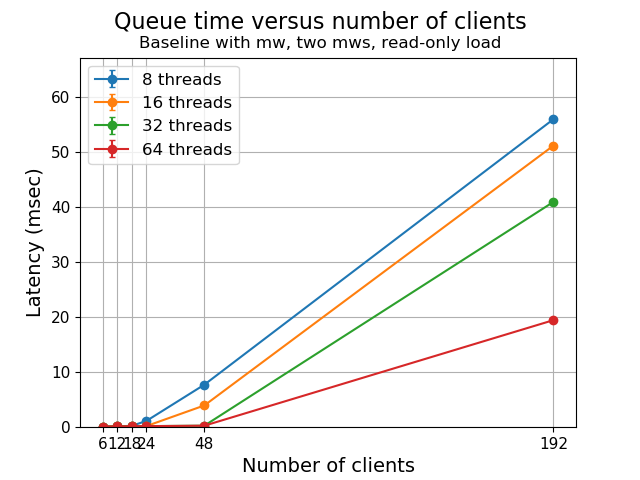
\includegraphics[width=1.0\linewidth,trim={5px 0px 20px 0px},clip]{img/plot/mwb2-ro-qtime_mw.png}
  \caption{Avg. queue time}
  \label{fig:mwb2-ro-qtime_mw}
\end{subfigure}
\caption{Average queue lengths and queue times for the read-only workload for baseline with middleware experiment with two middlewares.}
\label{fig:mwb2-ro-qstats}
\end{figure}

\subsubsection{Explanation} \label{sec:mwb2-exp}
Plots in Figures \ref{fig:mwb2-wo_mw} and \ref{fig:mwb2-wo-qstats} illustrate various statistics for the write-only load. We see results similar to the one middleware setup. System saturates at different number of clients for different number of worker threads. For the same average queue lengths, the queue times shorten as the number of worker threads increases. Again the number of working threads is our limiting factor for the system performance. Thus, we conclude the middleware being the bottleneck for the write-only case with two middlewares. Again, we find it intuitive that the statistics for the one middleware setup matches those of the two middleware setup with the half amount of worker threads, as it was the case with the read-only workload.
\par An intuitive correlation is as follows: statistics for the 8, 16 and 32 thread configurations for two middleware setup matches respectively with the 16, 32 and 64 thread settings for the one middleware. In other words, doubling the number of threads for one midleware has the same effects as introducing another middleware with the same number of threads on the system. Although, we can only say that for our experimental setup and configurations and this equivalence may not hold for factors much greater than two.
\par Results for the read-only workload is almost exactly the same as those from the setting with one middleware, as the bottleneck of the system is stays the same, which was detailed in the previous sections. Both the throughput and latency values (Figure \ref{fig:mwb2-ro_mw}) with respect to number of clients is quite similar to those of the configuration with one server, stemming from the same limitations.
\par Figure \ref{fig:mwb2-ro-qstats} illustrates the average queue length and queue time statistics for this experiment on read-only load. Here, we warn the reader to be careful when comparing the queue lengths for two and one middleware setups directly as the reported queue length is averaged over the middlewares. That is, to approximate the total number of requests waiting in the middleware queues one should multiply the averaged value by the number of middlewares in the environment. Lastly, we note the relation between queue lengths and queue times is the same as in the one middleware setup.

\subsection{Summary} \label{sec:mwb-summary}
Tables \ref{tab:mwb1-summary} and \ref{tab:mwb2-summary} reports the results for the middleware experiments, respectively the one middleware and the two middleware setups. All of the results shown in the tables are from the 64 worker thread configuration of the respective experiments.

\begin{table}[h]
\centering
{Maximum throughput for one middleware.}
\begin{tabular}{|l|p{2.3cm}|p{2.3cm}|p{2.7cm}|p{2.3cm}|}
\hline                       & Throughput        & {\small Response time}      & {\small Avg. queue time} & Miss rate \\ 
\hline Reads: Meas. on mw       & $2969.3 \pm 1.5$  & $5.413 \pm 0.021$  & $0.406 \pm 0.011$  & $0.0095404$ \\ 
\hline Reads: Meas. on clients  & $2969.3 \pm 1.8$  & $8.083 \pm 0.004$  & n/a                & $0.0095287$ \\ 
\hline Writes: Meas. on mw      & $8264.1 \pm 17.5$ & $9.125 \pm 0.017$  & $2.740 \pm 0.015$  & n/a \\ 
\hline Writes: Meas. on clients & $8263.5 \pm 17.3$ & $11.628 \pm 0.026$ & n/a                & n/a \\ 
\hline 
\end{tabular}
\caption{Summary of the baseline with one middleware.} \label{tab:mwb1-summary}
\end{table}
\begin{table}[h]
\centering
{Maximum throughput for two middlewares.}
\begin{tabular}{|l|p{2.3cm}|p{2.3cm}|p{2.7cm}|p{2.3cm}|}
\hline                      & Throughput         & {\small Response time}      & {\small Avg. queue time} & Miss rate \\ 
\hline Reads: Meas. on mw       & $2964.3 \pm 0.3$   & $2.288 \pm 0.061$  & $0.181 \pm 0.001$  & $0.0093647$ \\ 
\hline Reads: Meas. on clients  & $2964.4 \pm 0.8$   & $6.077 \pm 0.002$  & n/a                & $0.0095260$ \\ 
\hline Writes: Meas. on mw      & $10566.1 \pm 59.6$ & $16.121 \pm 0.118$ & $4.557 \pm 0.039$  & n/a     \\ 
\hline Writes: Meas. on clients & $10566.4 \pm 59.6$ & $18.206 \pm 0.105$ & n/a                & n/a     \\ 
\hline 
\end{tabular}
\caption{Summary of the baseline with two middlewares.} \label{tab:mwb2-summary}
\end{table}
%\begin{wrapfigure}{L}{0.5\textwidth} 
%  \centering
%  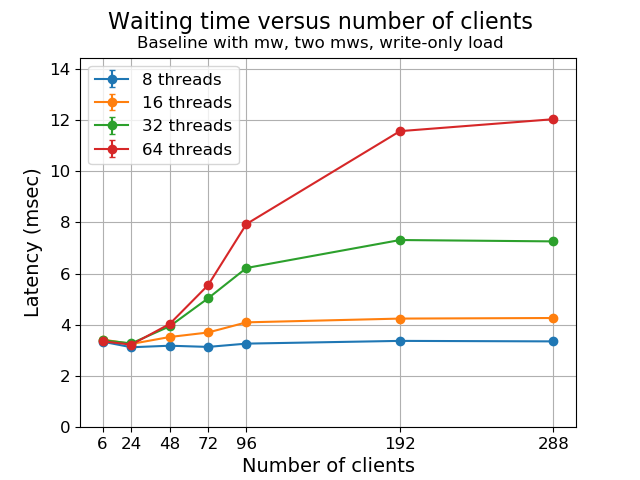
\includegraphics[width=1.0\linewidth,trim={5px 0px 20px 0px},clip]{img/plot/mwb2-wo-wtime_mw.png}
%  \caption{Server waiting times on write-only load for the baseline with middleware experiments with two middlewares}
%  \label{fig:mwb2-wo-wtime_mw}
%\end{wrapfigure}
\par First thing we can do is to compare the values aggregated by the clients with those obtained by the middlewares. Throughput and miss rate statistics show that they are approximately, but not absolutely, equal. As we aggregate data after cutting the warm-up and cool-down periods on both client and middleware outputs, this is a natural result. It is verified through additional experiments that the statistics match completely if the aggregations were to be done on the entirety of the data collected by both sides.
\par For response times, there is a significant but consistent difference between the averaged values reported by the middlewares and the clients. Client response times also include the time a request requires to travel from a client to a middleware and its reply from the middleware to the client, similarly. The difference between the aforementioned response times are equal to the round-trip time (RTT) of the clients and serves for the respective experiments. We can also observe that this RTT is not always constant. It is again natural as the network characteristics may fluctuate in between (and even during) experiments and we also employ multiple clients on different physical machines, we expect not a constant difference but a RTT that samples a probability distribution.
\par As discussed in Section \ref{sec:ov-methodology}, we populate the server with the 99\% of the keys we will use in the read-only experiments. This, in turn, (together with the fact that we do not allow any expiry) means that for each read-only experiment we should observe a miss rate around 1\% when looked from both middleware and client perspectives. Looking at the reported miss rates we can see that the values observed is in line with our expectations and client results corroborate the middleware aggregations. The marginal difference between values reported by clients and middlewares are due to times cut, as it is the case with throughput values.
\\
\par As explained in the preceding sections, maximum read-only throughput is just under 3000 requests per second, for both experiments. As the system is network bound under read-only load, changes in the number of middleware and the number of worker threads per middleware change neither where the system saturates, nor the maximum throughput achieved. Write-only experiments present us with a different picture. As the bottleneck of the system is middleware for both configurations, we see an increase in the maximum throughput obtained when we add a new middleware to the environment. This holds true not only for the 64 thread configuration which gives the best performance but for all sizes of the worker-thread pool. Looking once again at the Figures \ref{fig:mwb1-wo_mw} and \ref{fig:mwb2-wo_mw} we can see the saturation points for all worker-thread configurations go up with respect to clients. To illustrate, one middleware with 16 worker threads is already saturated with 48 clients but with two middlewares of 16 threads we see a continuous increase lasting between 72 and 96 clients. As discussed before, doubling the the number of middlewares has approximately the same effects on the system performance as doubling the size of the worker-thread pools in middlewares.
\\
\par The reader may notice the performance of the system measured in average throughput does not double when we double the number of middleware threads, either by doubling directly in one machine or adding another middleware. Our system is neither an ideal nor a simple system, so we do not expect such strong correlations and there are a couple of reasons that hinder the performance gain with a high number of worker threads. We always configure our servers to work with one thread, so an increase in the number of worker threads translate into an increase in the number of server connections, which might not scale very well in the presence with one thread. Additional handicaps could be due to the limitations of the middleware machines as the higher number of threads will result in more overhead and context switches, which diverges the system from the ideal performance.
\par Similarly to what we have discussed earlier in the Section \ref{sec:mwb1-exp}, again in the two middleware setting we can observe the server waiting times increasing when there are more worker threads present in the system. The trend is similar with both workloads and in the presence of one and two middlewares. One such trend can also be observed in the next section, where we have almost an identical experimental setup. Figure \ref{fig:tpfw-wtime_mw} illustrates one such example for the throughput for writes experiments. It serves as another method of verification of system saturation as a saturated system that operates with maximum utilization is expected to have stable waiting times as increases in the number of clients should only affect the queueing times.
\par Lastly, we note that even with two middlewares of 64 threads we cannot reach the maximum throughput achieved without middleware in the environment. We say the parameter values explored through experiments of this section is not enough to obtain performances comparable to the ones in Section \ref{sec:csb1}. For the same number of clients, additional network delays incurred and the overhead of the middlewares result in lower performances with the systems with middlewares.
\change{I should talk about queueing times and response times here possibly}
\begin{figure}[h!]
\centering
\begin{subfigure}{.5\textwidth}
  \centering
  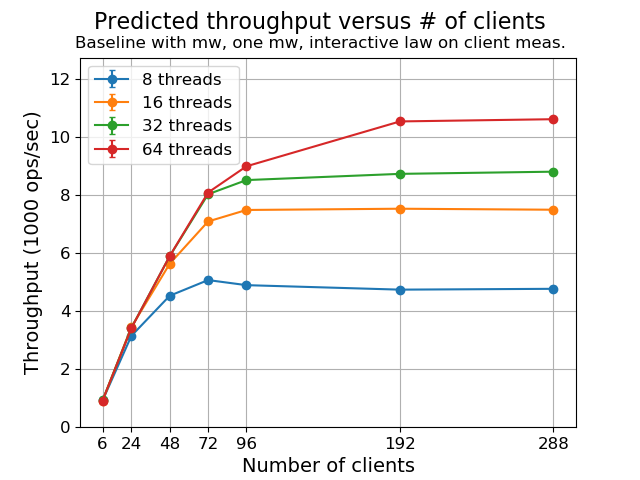
\includegraphics[width=1.0\linewidth,trim={5px 0px 20px 0px},clip]{img/plot/mwb2-wo-tp_law_cli.png}
  \caption{Predictions on client measurements}
  \label{fig:mwb2-wo-tp_law_cli}
\end{subfigure}%
\begin{subfigure}{.5\textwidth}
  \centering
  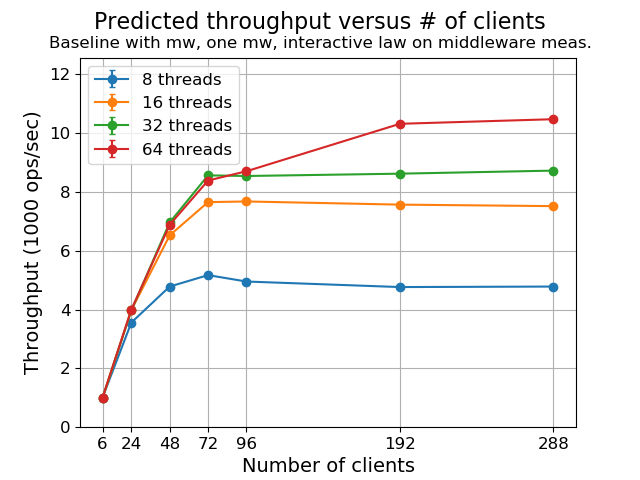
\includegraphics[width=1.0\linewidth,trim={5px 0px 20px 0px},clip]{img/plot/mwb2-wo-tp_law_mw.png}
  \caption{Predictions on adapted middleware measurements}
  \label{fig:mwb2-wo-tp_law_mw}
\end{subfigure}
\caption{Application of the interactive law illustrated for predictions made using client and midleware measurements. Each response time observed in middleware is increased by a constant amount to simulate the effects of RTT between clients and the middlewares. Results not being perfect indicate the RTT values are changing during experiments. These results show that RTT is not a constant value as in the ideal case, but it is a random variable.}
\label{fig:mwb2-wo-tp_law}
\end{figure}
\par Figure \ref{fig:mwb2-wo-tp_law_cli} provides an example illustration of the interactive law, reader should compare this plot with the actual values in Figure \ref{fig:mwb2-ro-tp_mw}. We only provide one exemplary plot here and the reader should feel free to use provided scripts and auxiliary plots to see the interactive law in action on other configurations that include middleware.
\par If we were to use the middleware measurements to predict the corresponding values, we would need to adapt the observed values. Our approach is to take the RTT between client and middleware machines as the think time of the clients when viewed from the perspective of the middleware. If we add the observed RTT times to the middleware response times for each experiment we would simply obtained the exact same results as ones with the client measurements. Instead, we also try modifying the middleware response times with an approximate RTT value for all experiments and the results can be still satisfactory. Figure \ref{fig:mwb2-wo-tp_law_mw} illustrates such a case (actual values again in Figure \ref{fig:mwb2-ro-tp_mw}). Reader can see some discrepancies between actual and the predicted values, which indicates the end-to-end delays not being constant for the duration of one experimental configuration, even using the same physical setup. Quite intuitively, we cannot perfectly estimate the actual throughput and response time values from the middleware observations without knowing the network conditions for that specific experiment.

\section{Throughput for Writes} \label{sec:tpfw}
This section inspects the system with three clients, two middlewares and three servers, under write-only load. Number of worker-threads and the number of clients are varied in order to understand the characteristic of the system through different configurations.

\subsection{Full System} \label{sec:tpfw-fs}
\begin{figure}[h!]
\centering
\begin{subfigure}{.5\textwidth}
  \centering
  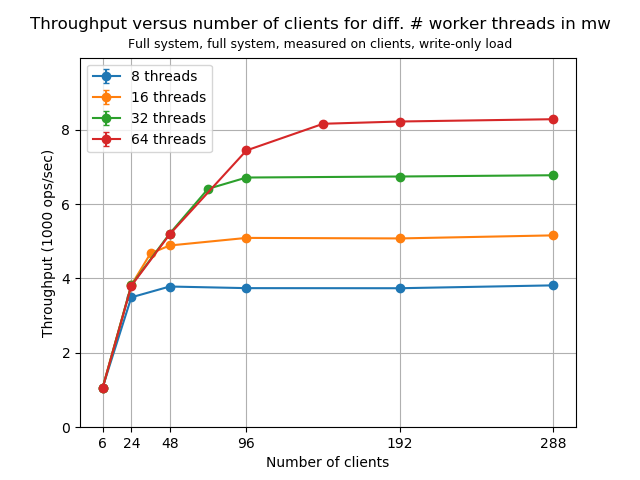
\includegraphics[width=1.0\linewidth,trim={5px 0px 20px 0px},clip]{img/plot/tpfw-tp_mw.png}
  \caption{Throughput}
  \label{fig:tpfw-tp_mw}
\end{subfigure}%
\begin{subfigure}{.5\textwidth}
  \centering
  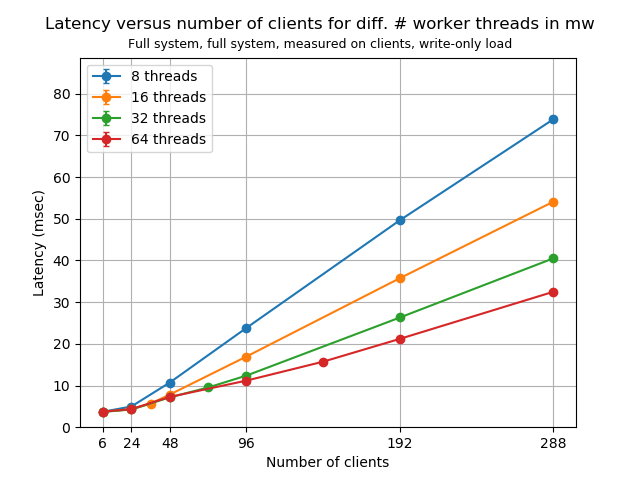
\includegraphics[width=1.0\linewidth,trim={5px 0px 20px 0px},clip]{img/plot/tpfw-lat_mw.png}
  \caption{Latency}
  \label{fig:tpfw-lat_mw}
\end{subfigure}
\caption{Throughput and latency values for the throughput for writes experiment, write-only workload.}
\label{fig:tpfw_mw}
\end{figure}

Figures \ref{fig:tpfw-tp_mw} and \ref{fig:tpfw-lat_mw} illustrate the average throughputs and response times of the system under different configurations. Each line represents a setup with a different number of threads for both plots. Results are similar to those analysed in Section \ref{sec:mwb2}, as the setup stays the same except the increase in the number of servers the system has. We see each configuration saturates at different points, since the middleware is the bottleneck of the system. Each of them conforms to the same trend: throughput gains become minimal and response times start to form a linear pattern as we move closer to the number of clients which saturates a given configuration. 

\begin{figure}[h!]
\centering
\begin{subfigure}{.5\textwidth}
  \centering
  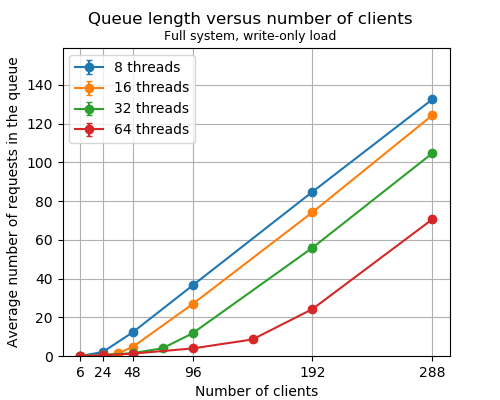
\includegraphics[width=1.0\linewidth,trim={5px 0px 20px 0px},clip]{img/plot/tpfw-qlen_mw.png}
  \caption{Avg. queue length}
  \label{fig:tpfw-qlen_mw}
\end{subfigure}%
\begin{subfigure}{.5\textwidth}
  \centering
  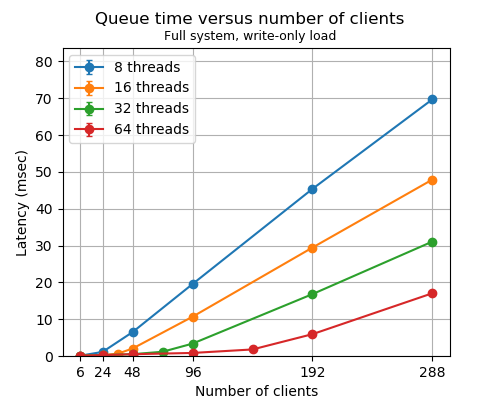
\includegraphics[width=1.0\linewidth,trim={5px 0px 20px 0px},clip]{img/plot/tpfw-qtime_mw.png}
  \caption{Avg. queue time}
  \label{fig:tpfw-qtime_mw}
\end{subfigure}
\caption{Average queue lengths and queue times for the throughput for writes experiment, write-only workload.}
\label{fig:tpfw_stats_mw}
\end{figure}

\subsubsection{Explanation} \label{sec:tpfw-exp}
\par For 8, 16, 32 and 64 worker-threads we state the saturation points are around 24, 36, 72 and 144 clients. With the exception of the 8 thread setup, we can see that the number of clients a saturated system can handle doubles as we double the worker-threads in the middleware. It is in line with our expectations as this ratio of number of worker-threads to the number of clients at the point of saturation should hold true for different number of worker threads with same configuration. Since middlewares are the bottlenecks of this setup, we except there should be enough requests in the systems waiting to be handled. This, in turn, means an increase in the number of worker-threads should amount to an approximately linear increase in the average number of requests that can be handled for a given period, which is indeed corroborated by the aforementioned results. Reader should note that the 8 worker thread setting has not the same level of granularity as the other settings and experiences a much sharper increase before leveling off. This points to the need for a finer grained search in the 6-24 client range, as the saturation of the 8 thread configuration is believed to be expected earlier than 24 clients, much likely around 18 clients considering the pattern described above.
\par Figures \ref{fig:tpfw-qlen_mw} and \ref{fig:tpfw-qtime_mw} respectively illustrate the average queue length and queueing time statistics for the throughput for writes experiment. As the experimental setup of this section is quite similar to the one in baseline experiments with two middlewares in Section \ref{sec:mwb2}, it is of no surprise that we obtain similar trends related to request queue. We can verify the saturation points for the different thread configurations as the points where lines in both plots become completely linear. We can again observe that corresponding lines in queue length and queue time plots have different slopes. For the system to reach a chosen queue length, we would need more clients with configurations with more threads. What that indicates is an increase in the number of threads in the middleware increases performance by reducing the queueing times, so the number of middleware threads is our limiting factor for this experiment.

\subsection{Summary} \label{sec:tpfw-summary}

\begin{table}[h]
\small
\centering
{Maximum throughput for the full system}
\begin{tabular}{|p{5.1cm}|p{2.1cm}|p{1.9cm}|p{1.9cm}|p{1.9cm}|}
\hline                                            & WT=8               & WT=16             & WT=32             & WT=64             \\ 
\hline Throughput (Middleware)                    & $3492.9 \pm 49.1$  & $4673.6 \pm 23.5$ & $6411.0 \pm 5.0$  & $8161.1 \pm 24.9$  \\ 
\hline Throughput (Derived from MW response time) & $3459.6 \pm 205.4$ & $4698.3 \pm 40.1$ & $6246.1 \pm 5.8$  & $8124.1 \pm 27.3$ \\ 
\hline Throughput (Client)                        & $3492.8 \pm 49.1$  & $4674.3 \pm 23.4$ & $6412.2 \pm 6.2$  & $8161.5 \pm 25.2$ \\ 
\hline Average time in queue                      & $1.112 \pm 0.062$  & $0.622 \pm 0.006$ & $1.148 \pm 0.010$ & $1.779 \pm 0.017$ \\ 
\hline Average length of queue                    & $2.0 \pm 0.0$      & $1.4 \pm 0.1$     & $4.0 \pm 0.2$     & $8.6 \pm 1.2$     \\ 
\hline Average time waiting for memcached         & $3.9 \pm 0.4$      & $5.0 \pm 0.1$     & $8.4 \pm 0.0$     & $13.9 \pm 0.0$    \\ 
\hline 
\end{tabular}
\caption{Summary of the throughput for writes experiments.} \label{tab:tpfw-summary}
\end{table}
\begin{figure}[h!]
\centering
\begin{subfigure}{.5\textwidth}
  \centering
  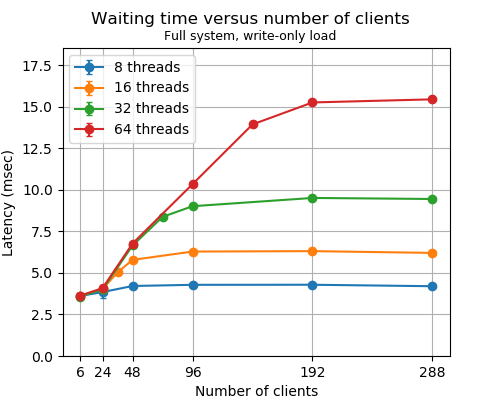
\includegraphics[width=1.0\linewidth,trim={5px 0px 10px 0px},clip]{img/plot/tpfw-wtime_mw.png}
  \caption{Server waiting times}
  \label{fig:tpfw-wtime_mw}
\end{subfigure}%
\begin{subfigure}{.5\textwidth}
  \centering
  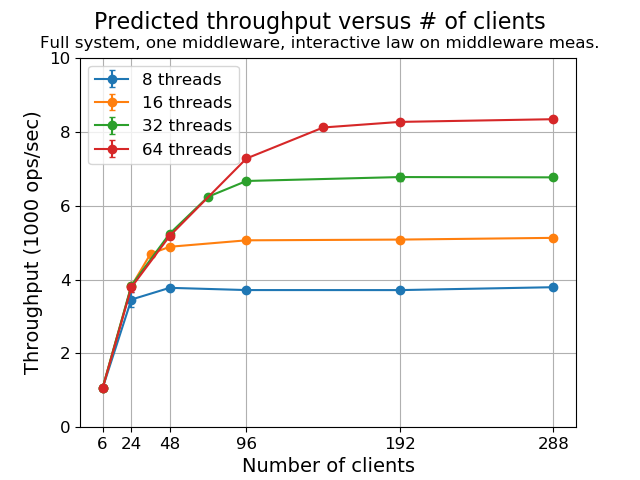
\includegraphics[width=1.0\linewidth,trim={5px 0px 10px 0px},clip]{img/plot/tpfw-tp_law_mw.png}
  \caption{Interactive law on middleware measurements}
  \label{fig:tpfw-tp_law_mw}
\end{subfigure}
\caption{Server waiting times and the application of the interactive law on the altered middleware measurements.}
\label{fig:tpfw-details}
\end{figure}
Table \ref{tab:tpfw-summary} presents a summary of the experiments of this section. Through the help of this table and the plots in Figure \ref{fig:auxiliary-2_mw} and \ref{fig:tpfw-details}, we will quickly go over the salient points of this experiment, many of which we have discussed before.
\par When we look into the reported maximum throughput values, we first verify the values reported by the clients and middlewares corroborate each other. The occasional differences are smaller than 0.1\% of the reported values and due to times cut for warm-up and cool-down periods, as discussed before in Section \ref{sec:mwb-summary}. The difference between the actual values and the ones derived using the interactive law is more apparent. Again, as discussed before in the aforementioned section, we first alter the middleware measurements to adapt them to the actual experimental setup. For that reason we take the average RTT between the clients and the middlewares to model the think time of the clients from the middleware perspective. Figure \ref{fig:tpfw-tp_law_mw} shows the overall results of this derivation, user should compare this plot to \ref{fig:tpfw-tp_mw}. It is of no surprise that the predicted values do not match our observations as we approximate the RTT between clients and middlewares as a constant, yet the end-to-end delay between different client and middleware machine pairs are different and they may even change as time passes.
\par Last thing regarding maximum throughput values we can mention is that improvement in the performance with the larger thread pools as the middlewares can serve more clients. However, one should note that the doubling the resources (e.g. number of middleware threads) does not always result in system performance (e.g. with respect to throughput) doubling. We argued about some possible underlying reasons and it is sensible that the change in the setup would not validate such claims. In fact, additional number of servers arises as another reason of why we cannot view the system as a black box and expect the changes in the system performance to be simple functions of its parameters.
\begin{figure}[h!]
\centering
\begin{subfigure}{.5\textwidth}
  \centering
  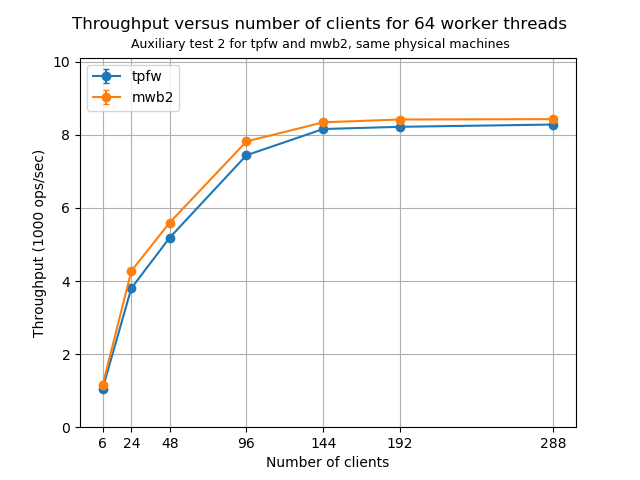
\includegraphics[width=1.0\linewidth,trim={5px 0px 10px 0px},clip]{img/plot/auxiliary-2-tp_mw.png}
  \caption{Throughput}
  \label{fig:auxiliary-2-tp_mw}
\end{subfigure}%
\begin{subfigure}{.5\textwidth}
  \centering
  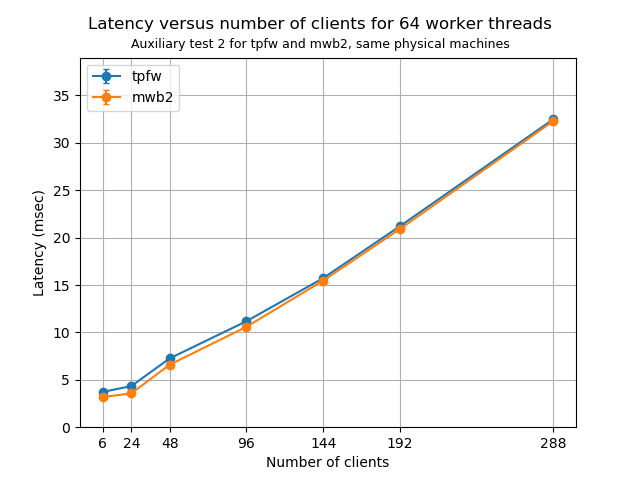
\includegraphics[width=1.0\linewidth,trim={5px 0px 10px 0px},clip]{img/plot/auxiliary-2-lat_mw.png}
  \caption{Latency}
  \label{fig:auxiliary-2-lat_mw}
\end{subfigure}
\caption{Throughput and latency values for an auxiliary experiment, write-only workload with 64 worker threads on middlewares. tpfw stands for the throughput for writes experiment, whereas the mwb2 denotes the middleware baseline experiment with two baselines.}
\label{fig:auxiliary-2_mw}
\end{figure}
\par We can see the average queue lengths for the points that give maximum throughput are minimal, resulting in negligible queueing times. It is also easy to see the higher number of threads can process the same queues faster by observing the queue time to queue length ratio decreasing with higher number of threads. Server waiting times presents us with another picture. We can see in Figure \ref{fig:tpfw-wtime_mw} the waiting times for different number of clients. Although it may not be as critical as the queueing times for the most cases, waiting times can be problematic for the configurations with many threads. As also discussed in Section \ref{sec:mwb-summary}, middlewares do their best to pop items from the queue and send them to the servers at the saturated regions. After saturation an increase in the number of clients will only result in an increase in the queue lengths as waiting times will not change as long as the middleware configuration is kept the same. Waiting times also serve as another tool for verifying our comments about saturation as we can see the saturation of the system as discussed earlier from another perspective.
\par As the experiments of this section and ones in the Section \ref{sec:mwb2} were conducted in different physical setups, it might not be satisfactory to compare them directly as we only expect minute differences in results. For this reason, we have conducted an auxiliary experiment which compares the configurations with same number of worker threads for these two experiments. Results can be viewed in Figure \ref{fig:auxiliary-2_mw}. The only difference between the configurations in this plot is the number of servers being 1 and 3. We expect the case with more servers to have a slightly lower performance than the other as sending requests to servers and waiting for their replies would incur some delays, even when it is being done in an asynchronous manner.

\section{Gets and Multi-gets} \label{sec:gmg}
This experiment again deals with the full system having 3 clients, 2 middlewares and 3 servers. Each of the two middleware has 8 worker threads and each client instance has one thread with two virtual clients (a total of 12 clients in the system). Clients send multi-get requests together with set requests and set to multi-get ratio for each experiment is 1:X where X is the number of keys in the multi-get requests. We change this key size and see how the system reacts. A comparative analysis is made on effects of the sharded and non-sharded aproaches for multi-get handling. Reader should feel free to take a look on Figure \ref{fig:flowchart}, which describes the operational flows for sharded and non-sharded cases.
\begin{figure}[h]
\begin{subfigure}{.5\textwidth}
  \centering
  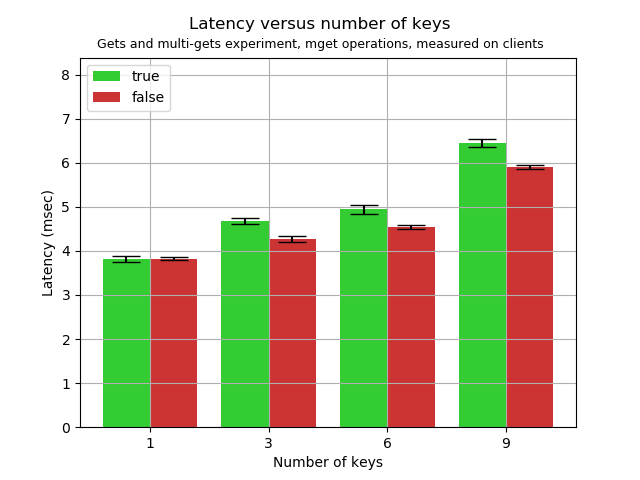
\includegraphics[width=1.0\linewidth ,trim={5px 0px 20px 0px},clip]{img/plot/gmg-mget-lat_cli.png}
  \caption{Response times}
  \label{fig:gmg-mget-lat_cli}
\end{subfigure}%
\begin{subfigure}{.5\textwidth}
  \centering
  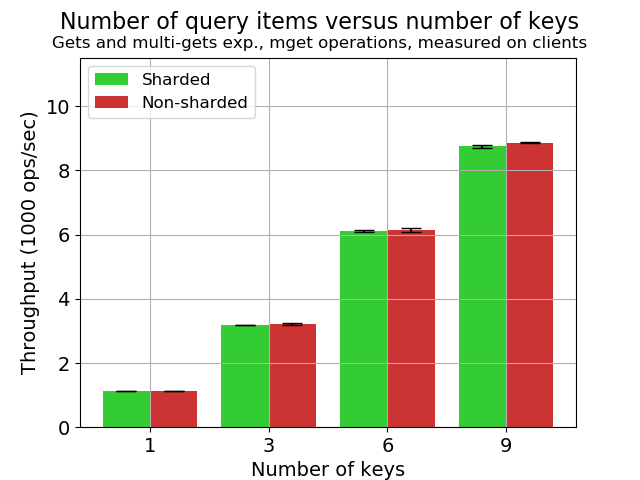
\includegraphics[width=1.0\linewidth ,trim={5px 0px 20px 0px},clip]{img/plot/gmg-mget-nitems_cli.png}
  \caption{Number of requested items}
  \label{fig:gmg-mget-nitems_cli}
\end{subfigure}
\caption{Response time and number of requested item statistics for sharded and non-sharded reads in different key size experiments}
\label{fig:gmg-mget_general}
\end{figure}

\subsection{Sharded Case} \label{sec:gmg-true}
In sharded case we split the multi-get requests send all splits to respective servers and proceed to listen for replies in the order we sent the requests. Illustrated in Figures \ref{fig:gmg-mget-lat_cli} and \ref{fig:gmg-mget-nitems_cli} we see the response times and number of requested items for expeirments with different key sizes. We define the number of requested items as total number of get queries sent through multi-get queries, that is, it is simply throughput times key size. We see both response times and number of requested items increasing as the key sizes grow larger. Figure \ref{fig:gmg-perc-true} shows the percentiles of the response time distribution for the sharded case. We can see each percentile value except the 99th increasing as the key sizes increase.

\subsubsection{Explanation} \label{sec:gmg-true-exp}
\par If we were to compare the response times observed with the ones in Section \ref{sec:mwb}, we can see that we get comparably larger response times for the same number of clients (12) as we now deal with a greater data flow throughout the system. Response times increase as the key sizes increase since larger requests result in more overhead in both middleware and server machines and accounts for larger end-to-end delays over the network.
\par We can verify in Figure \ref{fig:gmg-mget-nitems_cli} the number of individual get requests do not get close to 9000 requests, which was shown to be the upper limit due to bandwidth limitations in Sections \ref{sec:csb} and \ref{sec:mwb}. We say that we do not utilize the network in full efficiency, maybe except the 9 key case. If we were to continue increasing key cases in a similar fashion after the 9 key case, we believe we would not see any increase with respect to throughput as we would be already sending $\sim 9000$ requests back and forth. We also see the total number of requests are not perfectly  proportional to the key sizes as larger requests take more time in the system, resulting in smaller throughput per multi-get request.
\par We see for all key sizes that the average queue lengths and queueing times being approximately zero, although those statistics are not illustrated here due to space limitations. Then we can conclude the response time are only the results of the server waiting times as there are always worker threads available for the request handling. This shows the number of middleware threads is not a problem for any configuration as the queueing times are negligible everywhere.
\par We see the middleware worker threads being idle and network bandwidth not being a problem up to 9 key case, so we conclude the number of incoming requests are the limiting factor for us with the explored configurations. If the clients were sending more requests middleware would be able to relay them to the servers, achieving more throughput without causing long delays. 9 key case presents us with a different picture as it is where the system bottleneck changes: worker threads are still under saturated, but the system would not be able to handle any additional requests of same type as network is already fully utilized. It is intuitive that we would reach such a limit if we increase the request sizes without changing system parameters. Number of requests are the same and the additional overhead a larger multi-get causes is comparably small. Therefore, changing the key sizes create only small differences in middleware utilization but greatly effects the network usage.
\begin{figure}[h!]
\begin{subfigure}{.5\textwidth}
  \centering
  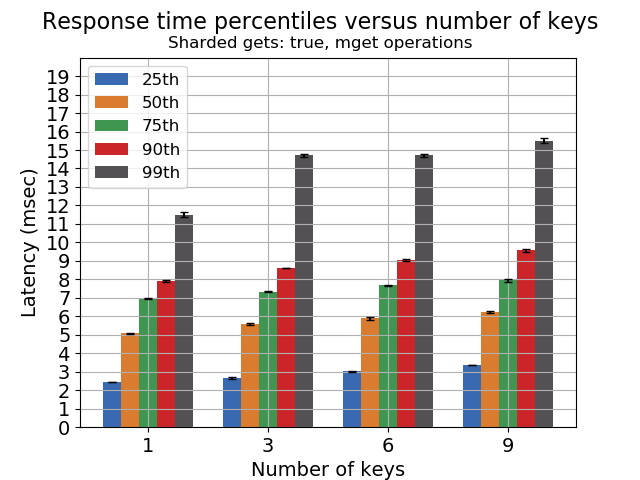
\includegraphics[width=1.0\linewidth ,trim={5px 0px 20px 0px},clip]{img/plot/gmg-perc-mget-true.png}
  \caption{Sharded case}
  \label{fig:gmg-perc-true}
\end{subfigure}%
\begin{subfigure}{.5\textwidth}
  \centering
  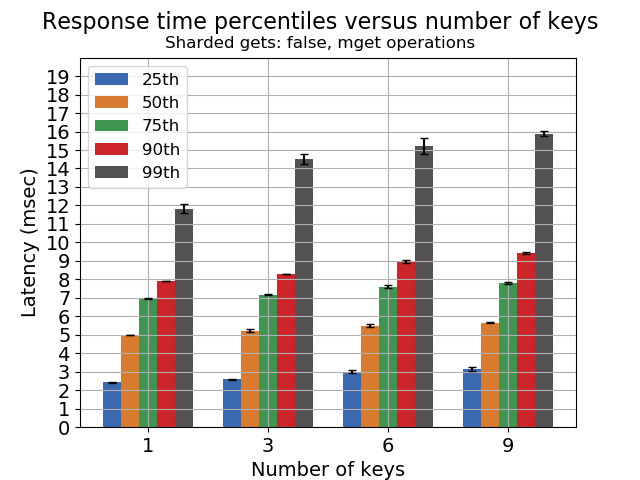
\includegraphics[width=1.0\linewidth ,trim={5px 0px 20px 0px},clip]{img/plot/gmg-perc-mget-false.png}
  \caption{Non-sharded case}
  \label{fig:gmg-perc-false}
\end{subfigure}
\caption{25th, 50th, 75th, 90th and 99th percentiles of sharded and non-sharded reads, for 1, 3, 6 and 9 key cases. Instead of their respective sections each, plots are provided side by side together to help the reader when comparing two cases.}
\label{fig:gmg-perc}
\end{figure}
Figure \ref{fig:gmg-perc-true} shows the percentiles of the response time distribution for the sharded reads. The results our in line with our expectations since we would expect most percentiles to go up as the key sizes grow larger. Assuming the network conditions are more or less the same in average and the overall system operates in a predictable and robust manner, each distinct request would have a bigger size, which in turn incur more network delays and both middleware and server overheads as discussed above. We cannot assert such a trend would be clearly visible in all percentiles as the extremal percentiles (99th for our case) only accumulate the extreme outliers which might not be representative of the general distribution of the response times. Such outliers indicate the extremal changes in the system states (be it internal or external, rather than the mean conditions. However, discrepancies between extremal percentiles would diminish more with more repetitions.

\subsection{Non-sharded Case} \label{sec:gmg-false}
Non-sharded case is rather straightforward as the worker threads of the middleware send the whole multi-get requests to only one server. The reader should remind the non-sharded case still utilizes a simple load-balancing scheme through round-robin as we have discussed earlier.

\subsubsection{Explanation} \label{sec:gmg-false-exp}
Figures \ref{fig:gmg-mget-lat_cli} and \ref{fig:gmg-mget-nitems_cli} show the response time and requested number of items statistics for the non-sharded case along with the sharded one. The trend in performance is quite similar to the one observed in sharded reads, which we have discussed earlier. Larger key sizes mean larger requests, which brings additional overhead in machines and latency over the network. Queue lengths are approximately zero and queueing times are negligible, again practically making the response times only a function of server waiting times (which incorporates both the service time of the servers and the RTT of the middleware-server connections). We again state the bottleneck is number of clients with respect to throughput and network bandwidth for the 9 key case only, with respect to total number of requested items.
\par We can see the non-sharded case consistently beating the sharded case in terms of throughput for the 1,3,6 and 9 key cases. Non-sharded case sends the whole data at once through one connection whereas the sharded case splits the data into three parts and sends it over three connections. Although the overall data sent through the network is same (excluding metadata of the network packages) utilizing multiple connections incur network overheads, both while sending the requests and receiving the replies. Therefore, it is no surprise that sharded reads have higher response times in average.
Figure \ref{fig:gmg-perc-false} illustrates the percentiles of the response time distribution for the non-sharded case. Similarly to the sharded case, percentiles go up as key size increases and we can even see this trend in the 99th percentiles of the non-sharded case. Non-sharded case almost consistently have smaller response times in all percentiles than the sharded one. This could be regarded as intuitive, since sharded reads cost additional latency per each request. We will not go into the details of the percentile plots here as it is hard to compare the trends for sharded and non-sharded percentiles in this range and we will discuss them alongside other topics in Section \ref{sec:gmg-summary}, where the results from additional experiments are explored together with the earlier ones.

\subsection{Histogram} \label{sec:gmg-hist}
\begin{figure}[h]
\begin{subfigure}{.5\textwidth}
  \centering
  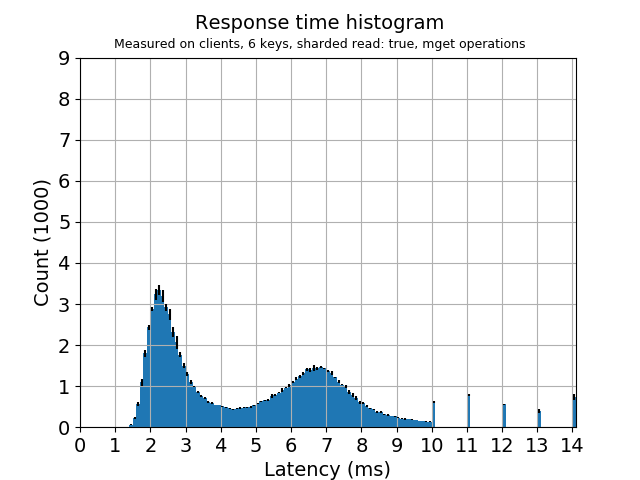
\includegraphics[width=1.0\linewidth ,trim={5px 0px 20px 0px},clip]{img/plot/gmg-hist6-true-mget_clients.png}
  \caption{Sharded case, client measurements}
  \label{fig:gmg-hist6-true-mget_clients}
\end{subfigure}%
\begin{subfigure}{.5\textwidth}
  \centering
  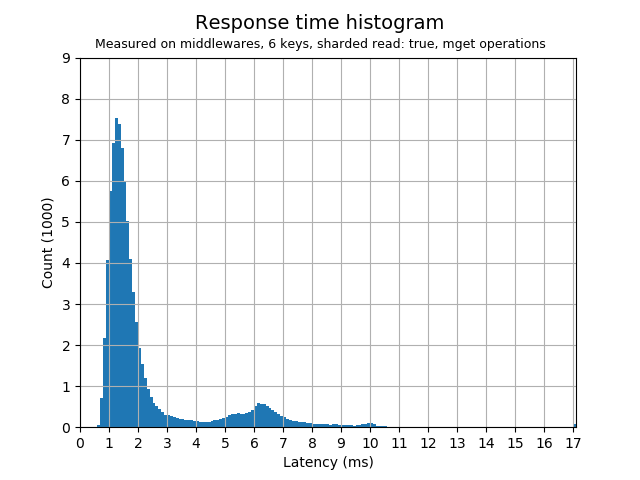
\includegraphics[width=1.0\linewidth ,trim={5px 0px 20px 0px},clip]{img/plot/gmg-hist6-true-mget_middlewares.png}
  \caption{Sharded case, middleware measurements}
  \label{fig:gmg-hist6-true-mget_middlewares}
\end{subfigure}
\begin{subfigure}{.5\textwidth}
  \centering
  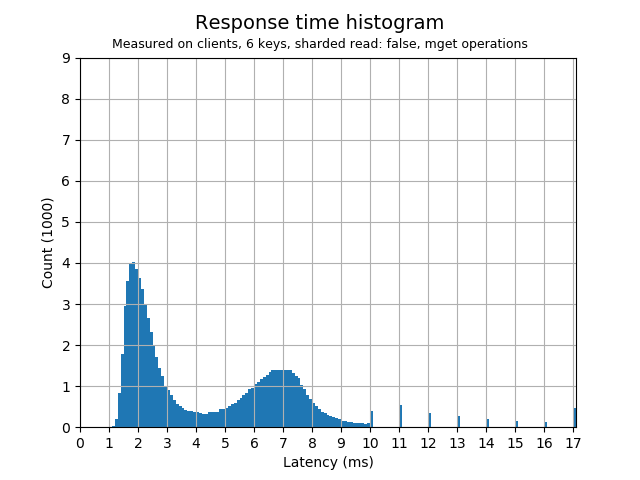
\includegraphics[width=1.0\linewidth ,trim={5px 0px 20px 0px},clip]{img/plot/gmg-hist6-false-mget_clients.png}
  \caption{Non-sharded case, client measurements}
  \label{fig:gmg-hist6-false-mget_clients}
\end{subfigure}%
\begin{subfigure}{.5\textwidth}
  \centering
  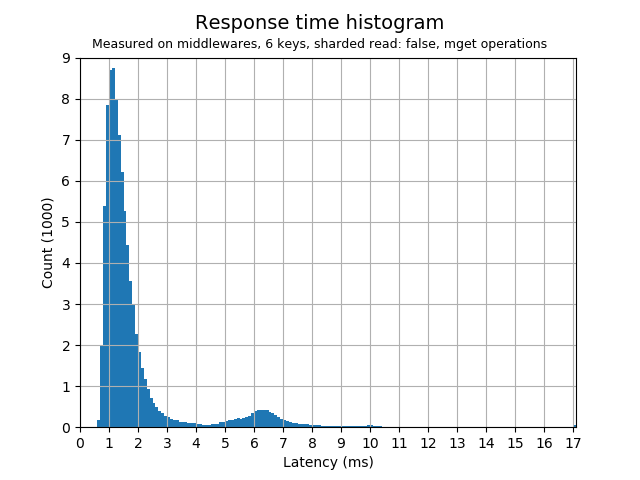
\includegraphics[width=1.0\linewidth ,trim={5px 0px 20px 0px},clip]{img/plot/gmg-hist6-false-mget_middlewares.png}
  \caption{Non-sharded case, middleware measurements}
  \label{fig:gmg-hist6-false-mget_middlewares}
\end{subfigure}
\caption{Response time distribution histograms for 6 key case. Bucket size is chosen as $100\mu s$ for all histograms, except for their last bins which contains the number of outlier response times that are greater than $16ms$. When choosing this cut-off value, it is ensured that less than 1\% of the occurrences are collected in the last bin for each individual result used in aggregation.}
\label{fig:gmg-hist6}
\end{figure}
Plots in Figure \ref{fig:gmg-hist6} show the response time histograms for the 6 keys case. These four plots illustrate the distribution of the response times for client and middleware measurements and under sharded and non-sharded read conditions. Histograms were constructed by aggregating all the response time in consecutive repeats, instead of averaging over them. This method of presentation was chosen in order to remove the clutter of error bars over histograms. Each histogram is inspected before to verify if the errors over repeats were negligible on each histogram constructed.
\par The most apparent characteristic of these pairs of plots is arguably the difference between the client and middleware histograms. Addition of the client-side latencies change the shape of the histograms by shifting the mass of response times to higher values. We attribute this difference mainly to the end-to-end delays between client and the middleware machines, although connection overheads in the middleware net-thread may also have some contribution to this additional latency. The reader should note that the response histograms do not just shift, but instead change their distribution. We may want to model the network as a delay center, but our observations indicate that the RTT between clients and middlewares are not constant as in the ideal case, but instead acts also as another queueing system. This is quite natural and we have also discussed this phenomenon in the earlier sections, especially when interpreting the predictions of the interactive law on altered middleware measurements (Figure \ref{fig:mwb2-wo-tp_law_mw} in Section \ref{sec:mwb-summary} and Figure \ref{fig:tpfw-tp_law_mw} in Section \ref{sec:tpfw-summary}). By the shape transformation we could argue that client-middleware RTT is skewed towards longer delays.
\\
\par Now, we compare the pairs of histograms for sharded and non-sharded read conditions. We can see in both pairs that the response time histograms for the sharded case are more sharply peaked than the non-sharded ones, and the non-sharded ones having fatter tails. The difference is especially evident in middleware histograms. As we discussed above, network conditions are not always the same and this result in end-to-end delays between machines fluctuating over time. By aggregating our observations we may diminish the effects of such fluctuations in our statistics but individually there could be significant differences between different requests. We also hinted at this issue while talking about the percentiles of the response time distribution (Figures \ref{fig:gmg-perc-true} and \ref{fig:gmg-perc-false}), stating such fluctuations were more visible in 99th percentiles than the others as they contain outlier values of a small sample size. This is essentially the reason why we see such a difference between the sharded and non-sharded reads.
\par Non-sharded ones send the complete request to one server, so it only experiences the end-to-end delay between a middleware and server, and only once. Network conditions may or may not be favorable when the data transfer happens, so the response time for that specific request should be expected to vary from time to time. Sharded read, on the other hand, splits the request into smaller parts and send them to different servers. Obviously this means we will have to experience more network delays in total, as we have noted earlier. However, by splitting the requests we diminish the effects of the network conditions between the middleware and the respective servers at the time the request is send and received. The way the sharded read sends smaller requests over the network further helps this, as the network conditions would be more observable in larger requests. Such conditions may or may not be favorable, so sharded case does not help requests to achieve a fast transfer \textemdash in fact, we are bound to wait the slowest connections to send and receive their respective split. We can observe this as the sharded histograms are slightly shifted to the right (higher response times) both location-wise and weight-wise. As the source of this difference is the middleware-server connections and how we choose to use the utilize these connections, difference between histograms being more visible in middleware histograms make sense. Client histograms lessen the effects of different read strategies by adding additional delays to both. Lastly, we claim the sharded reads tend to output more stable response time distribution but with the cost of additional delays.
\change{didn't talk about bimodal distributions at all, i suspect the reason for bimodal distr...}

%\begin{figure}[h]
%\begin{subfigure}{.5\textwidth}
%  \centering
%  \includegraphics[width=1.0\linewidth ,trim={0 0 0 0},clip]{img/gmg-hist6-true-mget.png}
%  \caption{Sharded case, client measurements}
%  \label{fig:gmg-hist6-true-mget_clients}
%\end{subfigure}
%\begin{subfigure}{.5\textwidth}
%  \centering
%  \includegraphics[width=1.0\linewidth ,trim={0 0 0 0},clip]{img/gmg-hist6-false-mget.png}
%  \caption{Non-sharded case, client measurements}
%  \label{fig:gmg-hist6-false-mget_clients}
%\end{subfigure}
%\caption{}
%\label{fig:gmg-hist6}
%\end{figure}

\subsection{Summary} \label{sec:gmg-summary}
\begin{figure}[h!]
\begin{subfigure}{.5\textwidth}
  \centering
  \includegraphics[width=1.0\linewidth ,trim={5px 0px 20px 0px},clip]{img/plot/gmg-extra-mget-lat_cli.png}
  \caption{Response times}
  \label{fig:gmg-extra-mget-lat_cli}
\end{subfigure}%
\begin{subfigure}{.5\textwidth}
  \centering
  \includegraphics[width=1.0\linewidth ,trim={5px 0px 20px 0px},clip]{img/plot/gmg-extra-mget-nitems_cli.png}
  \caption{Number of requested items}
  \label{fig:gmg-extra-mget-nitems_cli}
\end{subfigure}
\begin{subfigure}{.5\textwidth}
  \centering
  \includegraphics[width=1.0\linewidth ,trim={5px 0px 20px 0px},clip]{img/plot/gmg-extra-perc-mget-true.png}
  \caption{Sharded case}
  \label{fig:gmg-extra-perc-mget-true}
\end{subfigure}%
\begin{subfigure}{.5\textwidth}
  \centering
  \includegraphics[width=1.0\linewidth ,trim={5px 0px 20px 0px},clip]{img/plot/gmg-extra-perc-mget-false.png}
  \caption{Non-sharded case}
  \label{fig:gmg-extra-perc-mget-false}
\end{subfigure}
\caption{An auxiliary experiment for comparing sharded and non-sharded performances on multi-get requests with bigger key sets. Figures \ref{fig:gmg-extra-mget-lat_cli} and \ref{fig:gmg-extra-mget-nitems_cli} compare the average response time and number of requested items statistics for the sharded and non-sharded reads with 9, 18, 27, 54 and 81 key cases. Figures \ref{fig:gmg-extra-perc-mget-true} and \ref{fig:gmg-extra-perc-mget-false} illustrates 25th, 50th, 75th, 90th and 99th percentiles of sharded and non-sharded reads, for the experiments with aforementioned set of key sizes.}
\label{fig:gmg-extra}
\end{figure}
So far, we have discussed several aspects of the multi-get requests and the effects of different key sizes on sharded on non-sharded read strategies. Here, we inspect the experimental setup under larger key sizes to observe the trends in more detail. We test both strategies using 18, 27, 54 and 81 key sizes, on top of the 9 key case we have seen before. Results show that the our comments still hold true for bigger multi-get requests and we see other trends emerge. Plots in Figure \ref{fig:gmg-extra-perc-mget-false} show a summary of our auxiliary experiments with larger multi-get requests. These experiments are conducted on the same physical machines as the ones before, so reader should see them as natural extentions of the plots in Figures \ref{fig:gmg-mget_general} and \ref{fig:gmg-perc}.
\par Figure \ref{fig:gmg-extra-mget-lat_cli} compares the mean response times for the sharded and non-sharded experiments for the large key sizes. Response time differences become negligible in 54 keys and non-sharded response times become larger afterwards. We can see this trend from another perspective in Figure \ref{fig:gmg-extra-mget-nitems_cli}, where we see the 81 key case as the only configuration that has greater number of items requested for the sharded case than the non-sharded option. Bottleneck stays the same as in the 9 key case as we cannot see an increase in throughput (in terms of total get requests) as the system has already reached the network bandwidth. Queue lengths and queueing times are still negligible and the middleware is not fully utilized. We again turn our attention to the changing trend in the performance of sharded versus non-sharded reads in the light of this network limitation. As key sizes grow larger it becomes harder for the non-sharded case to allocate enough bandwidth to send big chunks of data across the network, whereas the sharded case can utilize server bandwidths more efficiently by requesting smaller replies from each server. For our case, this only becomes noticeable with comparably large key sizes, i.e. after 54 keyed multi-get requests. In a different setting, effects of network bandwidths could be more limiting and we can observe such changes with smaller key sizes (or vice versa with larger bandwidths).
\par Figures \ref{fig:gmg-extra-perc-mget-true} \ref{fig:gmg-extra-perc-mget-false} illustrate the percentiles of the response time distribution for the sharded and non-sharded configurations on larger key sizes. Unlike the smaller key sizes, we can see the different behaviours for two strategies more clearly where different percentiles scale much differently depending on the read strategy. 25th and 50th percentiles of the sharded reads are consistently greater than their non-sharded counterparts. This is not the case for the other ones as we see 75th percentiles favoring the sharded reads after 27 keys and 90th percentiles are always greater for the non-sharded reads. We talked about the inherent differences of two approaches in Section \ref{sec:gmg-hist}, where we have asserted that the sharded read approach results in more predictable response times but costs additional delays by doing so. This is corroborated by our percentile plots in this section as the underlying reasons are the same. Percentiles show that median response times are always smaller for the non-sharded read, confirming the sharded reads adds the requests more delay. Differences in other values show that the range of the response times are larger in the non-sharded reads. That is, fast replies are faster but the slow replies are slower in non-sharded reads. As the network conditions can fluctuate, non-sharded reads are effected (for better or for worse) more as they only use one connection at a time. We can see the mean and median differences in non-sharded case are larger and grow even more with larger key sizes. Overall, we see sharded reads generating more stable response times.
\par All in all, the preference of using one strategy over another may depend on the conditions and requirements of the system. It is harder to give reliable (or preferable) guarantees using non-sharded reads as they are affected more by the different conditions. We can give upper bounds for response times in sharded reads more easily, but this means we also report higher latencies. We suggest using sharded reads when dealing with large key sizes, limited bandwidths (e.g. in presence of network contention) and volatile or inconsistent network (or server) conditions. For our setting, it seems sensible to use sharding for multi-get requests that contain more than 54 keys, but the choice again depends on the tradeoff of having either smaller or more stable response times.

\section{2K Analysis} \label{sec:2k}
In this section, we perform a $2^{k}$ factorial analysis on three parameters: number of middlewares, number of servers and the number of worker threads per middleware. We believe the effects of these parameters are unidirectional, so $2^{k}$ factorial analysis suits our interests best. We solve the linear equation systems for both throughput and response times on both read-only and write-only workloads. Our aim is to assess the impacts of different parameters for different configurations, as well as further investigating and whether an additive or a multiplicative model would capture the interactions and variations in our system best.
\begin{table}[h]
\centering
\begin{tabular}{|l|c|c|c|c|}
\hline 
Parameter & Factor & Variable & {\small Value at min. (-1)} & {\small Value at max. (+1)} \\ 
\hline 
Number of middlewares & A & xA & 1 & 2 \\ 
\hline 
Number of servers & B & xB & 1 & 3 \\ 
\hline 
Worker threads per middleware & C & xC & 8 & 32 \\ 
\hline 
\end{tabular} 
\caption{$2^{k}$ experimental design used in this section, specifying the factors and treatments.} \label{tab:2k-factors}
\end{table}
\par Table \ref{tab:2k-factors} shows the system parameters and their corresponding variables and values chosen for the analyses. For each configurationon each workload, we solve two linear systems, which are illustrated in Equations \ref{eq:add-model} and \ref{eq:mult-model}. The former uses the assumption that the effects of the factors are additive, whereas the latter one assumes multiplicative effects. Equation for the multiplicative model is only different from the additive one in the sense that the take the response variables as logarithms of the observed values. In the scope of this section e denotes error whereas r denotes the number of repetitions. We use the response time and throughput values measured in client machines.
\begin{footnotesize}
\begin{equation} \label{eq:add-model}
y = q0 + qA*xA + qB*xB + qC*xC + qAB*xA*xB + qBC*xB*xC + qAC*xA*xC + qABC*xA*xB*xC + e
\end{equation}
\begin{equation} \label{eq:mult-model}
log(y) = q0 + qA*xA + qB*xB + qC*xC + qAB*xA*xB + qBC*xB*xC + qAC*xA*xC + qABC*xA*xB*xC + e
\end{equation}
\end{footnotesize}
\par Before going into the results of the analysis, it is good to know how the linear equations are formed and solved. Table \ref{tab:2k-example-table} shows an example of such equation systems, in this case the response variable being the throughput of the system on write-only load. Left part of the table is a sign table where $-1$'s refer to the minimum treatment and $+1$'s refer to the maximum treatment for a variable. We always conduct our factorial analyses with replications (so-called $2^{k}r$ design) so we solve our equations for the mean response (y\_mean) and estimate the errors in response values as e1, e2 and e3 over three repetitions. After solving the equation system we obtain the effects of the variables (e.g. qA for variable xA or qBC for variable interaction xB*xC) and calculate allocation of variation for each factor through sum of squares values. Equations \ref{eq:ssa}, \ref{eq:sse} and \ref{eq:sst} show how these calculations were done. The SSE accounts for the unexplained variation attributed to the experimental errors.
\begin{small}
\begin{equation} \label{eq:ssa}
SSA = 2^2 qA^2 \textnormal{, Fraction of variation explained (\%) by factor A} = SSA / SST
\end{equation}
\begin{equation} \label{eq:sse}
\textnormal{Sum of Squares for Error: } SSE = \sum_{i=1}^{2^{k}}\sum_{j=1}^{r} e_{ij}^{2} \textnormal{, Fraction of unexplained variation} = SSE / SST
\end{equation}
\begin{equation} \label{eq:sst}
\textnormal{Total Sum of Squares: } SST = SSA + SSB + SSC + SSAB + SSBC + SSAC + SSABC + SSE
\end{equation}
\end{small}
\begin{table}[h]
\centering
\begin{tabular}{|c|c|c|c|c|c|c|c|c|c|c|c|}
\hline
I & xA & xB & xC & {\small xA*xB} & {\small xB*xC} & {\small xA*xC} & {\small xA*xB*xC} & y\_mean & e1 & e2 & e3 \\ 
\hline
$1$ & $-1$ & $-1$ & $-1$ & $+1$ & $+1$ & $+1$ & $-1$ & 3364.3 & 45.56 & -15.33 & -30.23 \\
\hline
$1$ & $+1$ & $-1$ & $-1$ & $-1$ & $+1$ & $-1$ & $+1$ & 4318.9 & -19.85 & -1.77 & 21.63 \\
\hline
$1$ & $-1$ & $+1$ & $-1$ & $-1$ & $-1$ & $+1$ & $+1$ & 2655.2 & 23.47 & 37.06 & -60.54 \\
\hline
$1$ & $+1$ & $+1$ & $-1$ & $+1$ & $-1$ & $-1$ & $-1$ & 3729.6 & 9.09 & -39.41 & 30.32 \\
\hline
$1$ & $-1$ & $-1$ & $+1$ & $+1$ & $-1$ & $-1$ & $+1$ & 5832.8 & 6.49 & -17.43 & 10.93 \\
\hline
$1$ & $+1$ & $-1$ & $+1$ & $-1$ & $-1$ & $+1$ & $-1$ & 7321.3 & 17.68 & -21.73 & 4.04 \\
\hline
$1$ & $-1$ & $+1$ & $+1$ & $-1$ & $+1$ & $-1$ & $-1$ & 4786.4 & 27.09 & -18.71 & -8.38 \\
\hline
$1$ & $+1$ & $+1$ & $+1$ & $+1$ & $+1$ & $+1$ & $+1$ & 6782.0 & -16.40 & -2.95 & 19.35 \\
\hline
\end{tabular}
\caption{An example system of equations for the $2^{k}$ factorial analyses. Specifically, this set of equations with the corresponding y values model the throughput for the write-only load, assuming additive variable effects. Variable xA, xB and xC denote respectively the effects of number of middlewares, number of servers and the number of worker threads in our model.} \label{tab:2k-example-table}
\end{table}

Our principle reference for this chapter is Raj Jain's book \cite{book} on system performance analysis. It is argued that the \say{knowledge about the system behavior should always take precedence over statistical considerations}. As we are already familiar with the system through the different experimental setups in the previous sections, we do not view the system as a black box and rather choose the models that suits our parameter interactions best. For write-only workload we expect the factors xA (number of middlewares) and xC (number of threads per middleware) to be the important parameters, since our limiting factor is the total number of middleware threads in the system. As the total number of threads is the multiplication of these two factors and we expect the variation caused by the number of servers and the errors to be small, we choose multiplicative model for the write-only load. Similarly, with the read-only load we expect only the facor xB (number of servers) to be effective on the final results, so we choose the additive model as it also assumes the errors of the system are additive, not multiplicative.
\par Although we choose the models that fit the inner workings of our system, it is a good practice to model the system using both additive and multiplicative models (for both workloads and response variables) to see if there are any critical differences between two approaches. Respective results for the not chosen models are presented in the appendix part of this report, in Tables \ref{tab:2k-add-wo-tpt}, \ref{tab:2k-add-wo-lat}, \ref{tab:2k-mult-ro-tpt} and \ref{tab:2k-mult-ro-lat}. We see that the differences between additive and multiplicative models for all our analyses were not quite significant as both models essentially indicate the same results. There are several reasons behind this outcome. System is robust across repetitions and the residuals are low, thus modeling the errors one way or another does not affect the unexplained variation greatly. As it is also indicated in the book, \say{the logarithmic transformation is useful only if the ratio $y_{max}/y_{min}$ is large. For a small range the log function is almost linear, and so the analysis with the multiplicative model will produce results similar to that with the additive model}, which is exactly our case. Going from the additive to multiplicative model does not create a big difference in terms of the modelling power.
\begin{table}[h]
\centering
{Results of the additive model on read-only load}
\begin{minipage}{.5\textwidth}
\centering
	\begin{tabular}{|c|c|c|}
	\hline 
	{\small Source} & {\small Mean Estimate} & {\small Variation Expl. (\%)} \\ 
	\hline 
	qA & $265.8600$ & $0.009$ \\ 
	\hline 
	qB & $2678.2889$ & $0.944$ \\ 
	\hline 
	qC & $263.8299$ & $0.009$ \\ 
	\hline 
	qAB & $262.0704$ & $0.009$ \\ 
	\hline 
	qBC & $260.5430$ & $0.009$ \\ 
	\hline 
	qAC & $-257.6810$ & $0.009$ \\ 
	\hline 
	qABC & $-260.9624$ & $0.009$ \\ 
	\hline 
	% Error & \SI{1.05e-4} & $0.002$ \\ 
	% \hline 
	\end{tabular} \caption{Throughput analysis} \label{tab:2k-add-ro-tpt}
\end{minipage}%
\begin{minipage}{.5\textwidth}
\centering
	\begin{tabular}{|c|c|c|}
	\hline 
	{\small Source} & {\small Mean Estimate} & {\small Variation Expl. (\%)} \\ 
	\hline 
	qA & $-0.0009$ & $0.002$ \\ 
	\hline 
	qB & $-0.0208$ & $0.988$ \\ 
	\hline 
	qC & $-0.0009$ & $0.002$ \\ 
	\hline 
	qAB & $-0.0009$ & $0.002$ \\ 
	\hline 
	qBC & $-0.0009$ & $0.002$ \\ 
	\hline 
	qAC & $0.0009$ & $0.002$ \\ 
	\hline 
	qABC & $0.0009$ & $0.002$ \\ 
	\hline 
	% Error & \SI{1.18e-09} & $0.001$ \\ 
	% \hline 
	\end{tabular} \caption{Latency analysis} \label{tab:2k-add-ro-lat}
\end{minipage}
\end{table}\label{tab:2k-add-ro}
\\
\par Now we turn our attention to the findings of the models. We present the mean estimate of the parameters and the percentage of variation in the response variable explained by the variation of those parameters for analyses on throughput and latency over read-only and write-only workloads. Tables \ref{tab:2k-add-ro-tpt} and \ref{tab:2k-add-ro-lat} show the results for the read-only load. Clearly, the only important factor is the number of servers in the system while the other factors and factor interactions are equally unimportant. Analyses on both throughput and latency corroborate each other: number of servers have a strong positive influence on the throughput and a strong negative influence on the response time values. As we have discussed this issue on Sections \ref{sec:csb} and \ref{sec:mwb}, network bandwidth is the bottleneck for the read-only load most of the time. Our choice of minimum and maximum treatments for each factor (Table \ref{tab:2k-factors}) results in number of servers being the bottleneck in every experiment except the 8 thread total with 3 servers case. This is in line with our expectations and findings in previous sections. Percentage of unexplained variation due to errors amount to $0.002$ and $0.001$, respectively for throughput and response time analyses. Therefore, we rule out the effects of sources other than the number of servers, including the error, as their variation does not really change values of the response variable.
\begin{table}[h]
\centering
{Results of the multiplicative model on write-only load}
\begin{minipage}{.5\textwidth}
\centering
	\begin{tabular}{|c|c|c|}
	\hline 
	{\small Source} & {\small Mean Estimate} & {\small Variation Expl. (\%)} \\ 
	\hline 
	qA & $0.1457$ & $0.194$ \\ 
	\hline 
	qB & $-0.0822$ & $0.062$ \\ 
	\hline 
	qC & $0.2832$ & $0.733$ \\ 
	\hline 
	qAB & $0.0264$ & $0.006$ \\ 
	\hline 
	qBC & $0.0137$ & $0.002$ \\ 
	\hline 
	qAC & $-0.0017$ & $0.000$ \\ 
	\hline 
	qABC & $0.0039$ & $0.000$ \\ 
	\hline 
	% Error & \SI{7.87e-05} & $0.003$ \\ 
	% \hline 
	\end{tabular} \caption{Throughput analysis} \label{tab:2k-mult-wo-tpt}
\end{minipage}%
\begin{minipage}{.5\textwidth}
\centering
	\begin{tabular}{|c|c|c|}
	\hline 
	{\small Source} & {\small Mean Estimate} & {\small Variation Expl. (\%)} \\ 
	\hline 
	qA & $-0.1384$ & $0.165$ \\ 
	\hline 
	qB & $0.0963$ & $0.080$ \\ 
	\hline 
	qC & $-0.2730$ & $0.642$ \\ 
	\hline 
	qAB & $-0.0192$ & $0.003$ \\ 
	\hline 
	qBC & $-0.0031$ & $0.000$ \\ 
	\hline 
	qAC & $0.0124$ & $0.001$ \\ 
	\hline 
	qABC & $0.0065$ & $0.000$ \\ 
	\hline 
	% Error & \SI{1.35e-09} & $0.108$ \\ 
	% \hline 
	\end{tabular} \caption{Latency analysis} \label{tab:2k-mult-wo-lat}
\end{minipage}
\end{table}\label{tab:2k-mult-wo}
\par For the write-only workload we expect the total number of worker threads to have a strong effect on system performance such that more worker threads should correspond to higher throughput and lower response time values. Similarly, we believe the number of servers for write-only workloads should hinder the system performance, perhaps not as noticeably as with the total number of threads. We first send the queries to all servers and then wait for their responses. That way we do not experience the RTT for all the servers, although the time a worker thread waits increases linearly with the number of servers. In the optimistic case, reply from the first server would arrive as we finish sending the query to last server.
\par In Tables \ref{tab:2k-mult-wo-tpt} and \ref{tab:2k-mult-wo-lat} we can see the factorial analysis results for the write-only workload. Number of middlewares and the number of threads per middleware together account for the vast majority of the variation for both throughput and latency as expected. The reason that the variation due to number of threads per middleware (xC) is greater than that of the number of middlewares (xA) should not be surprising as the min-max values for xC covers a greater change than the xA, with respect to total number of threads (Table \ref{tab:2k-factors}). We can also see xB having a slightly negative influence on throughput (vice versa for response times) since the number of servers only affect the performance marginally, as we have demonstrates in Section \ref{sec:tpfw-summary} with the help of findings shown in Figure \ref{fig:auxiliary-2_mw}. Unexplained variations ($0.003$ and $0.108$ for throughput and response times, respectively) for the write-only load is greater than those for the read-only load, since the system conditions (e.g. end-to-end delays between physical machine pairs) have an effect on the performance of the system in the observed value ranges. It was not the case with the read-only workload as the network bandwidth limited the performance such that changing the number of threads in our range did not change the bottleneck being the bandwidth.

\section{Queuing Model} \label{sec:queueing-model}
\begin{table}[h]
\begin{minipage}{.5\textwidth}
	\centering
	\begin{tabular}{|l|c|}
		\hline $\rho$		& Traffic intensity					\\
		\hline $E[n]$		& Mean num. of jobs in the system	\\
		\hline $E[n_{q}]$	& Mean num. of jobs in the queue 	\\
		\hline $E[r]$		& Mean response time					\\
		\hline $E[w]$		& Mean waiting time					\\
		\hline 
	\end{tabular}
\end{minipage}%
\begin{minipage}{.5\textwidth}
	\centering
	\begin{tabular}{|l|c|}
		\hline $\lambda$		& Arrival rate						\\
		\hline qlen			& Avg. queue length per middleware	\\
		\hline $2\times$qlen	& Avg. queue length of the system	\\
		\hline qtime			& Avg. queueing time					\\
		\hline wtime			& Avg. server waiting time			\\
		\hline 
	\end{tabular}
\end{minipage}
\caption{Notation used throughout this section} \label{tab:queueing-notation}
\end{table}	

\subsection{M/M/1} \label{sec:mm1}
We isolate system from the middleware perspective and try to model the system using middleware measurements. We determine a service rate for each number of worker threads and construct a different M/M/1 model for that specific configuration. Tables \ref{tab:mm1-8}, \ref{tab:mm1-16}, \ref{tab:mm1-32} and \ref{tab:mm1-64} show the results for the models constructed for 8, 16, 32 and 64 threads, respectively. We consider the maximum throughput achieved by a specific configuration indicates its maximal capacity and choose that value as the service rate for that configuration. By constructing and testing our models we use the data obtained through the experiments in Section \ref{sec:tpfw}.
\begin{table}[h]
\centering
\begin{tabular}{|c|c|c|c|c|c|c|c|c|c|c|}
\hline
num & \multicolumn{6}{ |c| }{Model outputs} & \multicolumn{4}{ |c| }{Middleware meas.} \\
\cline{2-11}
Cli & $\lambda$ & $\rho$ & $E[n]$ & $E[n_{q}]$ & $E[r]$ & $E[w]$ & qlen & $2\times$qlen & qtime & wtime \\
\hline
6 & 1060.2 & 0.278 & 0.385 & 0.107 & 0.36 & 0.10 & 0.0 & 0.0 & 0.078 & 3.6 \\
\hline
24 & 3492.9 & 0.916 & 10.8 & 9.9 & 3.11 & 2.84 & 2.0 & 4.0 & 1.11 & 3.9 \\
\hline
48 & 3783.7 & 0.992 & 121.3 & 120.3 & 32.05 & 31.79 & 12.2 & 24.4 & 6.49 & 4.2 \\
\hline
96 & 3740.3 & 0.980 & 50.1 & 49.2 & 13.41 & 13.14 & 36.4 & 72.8 & 19.54 & 4.3 \\
\hline
192 & 3737.8 & 0.979 & 48.5 & 47.5 & 12.97 & 12.71 & 84.8 & 169.6 & 45.38 & 4.3 \\
\hline
\end{tabular}
\caption{Results of the M/M/1 model for the 8 worker thread configuration. All time values are given in milliseconds. Service rate is $\mu = 3814.9$, which is the absolute maximum throughput this configuration can achieve.}
\label{tab:mm1-8}
\end{table}

\begin{table}[h]
\centering
\begin{tabular}{|c|c|c|c|c|c|c|c|c|c|c|}
\hline
num & \multicolumn{6}{ |c| }{Model outputs} & \multicolumn{4}{ |c| }{Middleware meas.} \\
\cline{2-11}
Cli & $\lambda$ & $\rho$ & $E[n]$ & $E[n_{q}]$ & $E[r]$ & $E[w]$ & qlen & $2\times$qlen & qtime & wtime \\
\hline
6 & 1056.0 & 0.205 & 0.257 & 0.0527 & 0.24 & 5e-02 & 0.1 & 0.2 & 0.079 & 3.6 \\
\hline
24 & 3823.2 & 0.741 & 2.86 & 2.12 & 0.748 & 0.555 & 0.4 & 0.8 & 0.246 & 4.0 \\
\hline
36 & 4673.6 & 0.906 & 9.62 & 8.71 & 2.06 & 1.86 & 1.4 & 2.8 & 0.622 & 5.0 \\
\hline
48 & 4887.3 & 0.947 & 17.96 & 17.01 & 3.67 & 3.48 & 4.6 & 9.2 & 2.02 & 5.8 \\
\hline
96 & 5091.2 & 0.987 & 74.65 & 73.66 & 14.66 & 14.47 & 26.8 & 53.6 & 10.66 & 6.3 \\
\hline
192 & 5077.2 & 0.984 & 61.77 & 60.78 & 12.16 & 11.97 & 74.2 & 148.4 & 29.44 & 6.3 \\
\hline
\end{tabular}
\caption{Results of the M/M/1 model for the 16 worker thread configuration. All time values are given in milliseconds. Service rate is $\mu = 5159.4$, which is the absolute maximum throughput this configuration can achieve.}
\label{tab:mm1-16}
\end{table}

\begin{table}[h]
\centering
\begin{tabular}{|c|c|c|c|c|c|c|c|c|c|c|}
\hline
num & \multicolumn{6}{ |c| }{Model outputs} & \multicolumn{4}{ |c| }{Middleware meas.} \\
\cline{2-11}
Cli & $\lambda$ & $\rho$ & $E[n]$ & $E[n_{q}]$ & $E[r]$ & $E[w]$ & qlen & $2\times$qlen & qtime & wtime \\
\hline
6 & 1046.8 & 0.154 & 0.183 & 0.028 & 0.174 & 2.7e-02 & 0.0 & 0.0 & 0.083 & 3.6 \\
\hline
24 & 3823.6 & 0.564 & 1.29 & 0.73 & 0.339 & 0.191 & 0.4 & 0.8 & 0.237 & 4.0 \\
\hline
48 & 5206.5 & 0.768 & 3.32 & 2.55 & 0.636 & 0.489 & 1.5 & 3.0 & 0.494 & 6.7 \\
\hline
72 & 6411.0 & 0.946 & 17.53 & 16.58 & 2.73 & 2.59 & 4.0 & 8.0 & 1.148 & 8.4 \\
\hline
96 & 6715.1 & 0.991 & 109.0 & 108.0 & 16.23 & 16.09 & 11.7 & 23.4 & 3.363 & 9.0 \\
\hline
192 & 6742.6 & 0.995 & 197.7 & 196.7 & 29.32 & 29.18 & 55.9 & 111.8 & 16.806 & 9.5 \\
\hline
\end{tabular}
\caption{Results of the M/M/1 model for the 32 worker thread configuration. All time values are given in milliseconds. Service rate is $\mu = 6776.7$, which is the absolute maximum throughput this configuration can achieve.}
\label{tab:mm1-32}
\end{table}

\begin{table}[h]
\centering
\begin{tabular}{|c|c|c|c|c|c|c|c|c|c|c|}
\hline
num & \multicolumn{6}{ |c| }{Model outputs} & \multicolumn{4}{ |c| }{Middleware meas.} \\
\cline{2-11}
Cli & $\lambda$ & $\rho$ & $E[n]$ & $E[n_{q}]$ & $E[r]$ & $E[w]$ & qlen & $2\times$qlen & qtime & wtime \\
\hline
6 & 1045.4 & 0.126 & 0.144 & 0.018 & 0.138 & 1.7e-02 & 0.0 & 0.0 & 0.084 & 3.6 \\
\hline
24 & 3803.6 & 0.459 & 0.849 & 0.389 & 0.2233 & 0.102 & 0.3 & 0.6 & 0.250 & 4.1 \\
\hline
48 & 5187.8 & 0.626 & 1.675 & 1.05 & 0.323 & 0.202 & 1.2 & 2.4 & 0.484 & 6.8 \\
\hline
96 & 7443.5 & 0.898 & 8.857 & 7.96 & 1.19 & 1.07 & 3.9 & 7.8 & 0.829 & 10.4 \\
\hline
144 & 8161.1 & 0.985 & 66.46 & 65.47 & 8.14 & 8.02 & 8.6 & 17.2 & 1.779 & 13.9 \\
\hline
192 & 8221.8 & 0.992 & 132.4 & 131.4 & 16.10 & 15.98 & 24.2 & 48.4 & 5.932 & 15.3 \\
\hline
\end{tabular}
\caption{Results of the M/M/1 model for the 64 worker thread configuration. All time values are given in milliseconds. Service rate is $\mu = 8283.9$, which is the absolute maximum throughput this configuration can achieve.}
\label{tab:mm1-64}
\end{table}

\subsection{M/M/m} \label{sec:mmm}
\begin{table}[h]
\centering
\begin{tabular}{|c|c|c|c|c|c|c|c|c|c|c|}
\hline
num & \multicolumn{6}{ |c| }{Model outputs} & \multicolumn{4}{ |c| }{Middleware meas.} \\
\cline{2-11}
Cli & $\lambda$ & $\rho$ & $E[n]$ & $E[n_{q}]$ & $E[r]$ & $E[w]$ & qlen & $2\times$qlen & qtime & wtime \\
\hline
6 & 1056.0 & 0.510 & 8.17 & 0.011 & 7.74 & 1.1e-02 & 0.1 & 0.2 & 0.079 & 3.6 \\
\hline
\end{tabular}
\caption{Results of the M/M/m model for the 16 worker thread configuration. All time values are given in milliseconds. Service rate is $\mu = 129.4359375$, which is the absolute maximum throughput per thread of the 64 thread configuration.}
\label{tab:mmm-16_64}
\end{table}

\begin{table}[h]
\centering
\begin{tabular}{|c|c|c|c|c|c|c|c|c|c|c|}
\hline
num & \multicolumn{6}{ |c| }{Model outputs} & \multicolumn{4}{ |c| }{Middleware meas.} \\
\cline{2-11}
Cli & $\lambda$ & $\rho$ & $E[n]$ & $E[n_{q}]$ & $E[r]$ & $E[w]$ & qlen & $2\times$qlen & qtime & wtime \\
\hline
6 & 1046.8 & 0.253 & 8.087 & $\sim 0$ & 7.73 & $\sim 0$ & 0.0 & 0.0 & 0.083 & 3.6 \\
\hline
24 & 3823.6 & 0.923 & 36.2 & 6.73 & 9.48 & 1.76 & 0.4 & 0.8 & 0.237 & 4.0 \\
\hline
\end{tabular}
\caption{Results of the M/M/m model for the 32 worker thread configuration. All time values are given in milliseconds. Service rate is $\mu = 129.4359375$, which is the absolute maximum throughput per thread of the 64 thread configuration.}
\label{tab:mmm-32_64}
\end{table}

\begin{table}[h]
\centering
\begin{tabular}{|c|c|c|c|c|c|c|c|c|c|c|}
\hline
num & \multicolumn{6}{ |c| }{Model outputs} & \multicolumn{4}{ |c| }{Middleware meas.} \\
\cline{2-11}
Cli & $\lambda$ & $\rho$ & $E[n]$ & $E[n_{q}]$ & $E[r]$ & $E[w]$ & qlen & $2\times$qlen & qtime & wtime \\
\hline
6 & 1045.4 & 0.126 & 8.08 & $\sim 0$ & 7.726 & $\sim 0$ & 0.0 & 0.0 & 0.084 & 3.6 \\
\hline
24 & 3803.6 & 0.459 & 29.4 & $\sim 0$ & 7.726 & $\sim 0$ & 0.3 & 0.6 & 0.250 & 4.1 \\
\hline
48 & 5187.8 & 0.626 & 40.1 & $\sim 0$ & 7.726 & $\sim 0$ & 1.2 & 2.4 & 0.484 & 6.8 \\
\hline
96 & 7443.5 & 0.898 & 60.2 & 2.7 & 8.09 & 0.362 & 3.9 & 7.8 & 0.829 & 10.4 \\
\hline
144 & 8161.1 & 0.985 & 120.4 & 57.3 & 14.75 & 7.02 & 8.6 & 17.2 & 1.779 & 13.9 \\
\hline
192 & 8221.8 & 0.992 & 186.5 & 122.9 & 22.68 & 14.96 & 24.2 & 48.4 & 5.932 & 15.3 \\
\hline
\end{tabular}
\caption{Results of the M/M/m model for the 64 worker thread configuration. All time values are given in milliseconds. Service rate is $\mu = 129.4359375$, which is the absolute maximum throughput per thread of the 64 thread configuration.}
\label{tab:mmm-64_64}
\end{table}

\subsection{Network of Queues} \label{sec:network-of-queues}
\maybe{You need to consider both 1 and 2 middleware configuration. You need to analyse both read only and write only workloads. You can set the number of worker threads to the constant that delivers highest throughput.}

\begin{thebibliography}{9}
\bibitem{memcached} Memcached: a distributed memory object caching system \url{https://memcached.org/}
\bibitem{memtier} memtier\_benchmark: a high-throughput benchmarking tool for Redis \& Memcached \url{https://github.com/RedisLabs/memtier\_benchmark}
\bibitem{dstat} Dstat: a versatile resource statistics tool \url{http://dag.wiee.rs/home-made/dstat/}
\bibitem{iperf} iPerf: the TCP, UDP and SCTP network bandwidth measurement tool \url{https://iperf.fr/}
\bibitem{book} Jain, R. (1990). The art of computer systems performance analysis: techniques for experimental design, measurement, simulation, and modeling. John Wiley \& Sons.
\bibitem{cssh} Cluster SSH: cluster administration tool via SSH \url{https://github.com/duncs/clusterssh}
\end{thebibliography}

\clearpage

\section*{Appendix} \label{sec:appendix}

\subsubsection*{2K Analysis: additional tables} \label{sec:app-2k-analysis-add-plots}
\begin{table}[h]
\centering
{Results of the additive model on write-only load}
\begin{minipage}{.5\textwidth}
\centering
	\begin{tabular}{|c|c|c|}
	\hline 
	{\small Source} & {\small Mean Estimate} & {\small Variation Expl. (\%)} \\ 
	\hline 
	qA & $689.1529$ & $0.196$ \\ 
	\hline 
	qB & $-360.4905$ & $0.054$ \\ 
	\hline 
	qC & $1331.8182$ & $0.731$ \\ 
	\hline 
	qAB & $78.3606$ & $0.003$ \\ 
	\hline 
	qBC & $-35.9031$ & $0.001$ \\ 
	\hline 
	qAC & $181.8770$ & $0.014$ \\ 
	\hline 
	qABC & $48.4125$ & $0.001$ \\ 
	\hline 
	% Error & \SI{1.18e-4} & $0.002$ \\ 
	% \hline 
	\end{tabular} \caption{Throughput analysis} \label{tab:2k-add-wo-tpt}
\end{minipage}%
\begin{minipage}{.5\textwidth}
\centering
	\begin{tabular}{|c|c|c|}
	\hline 
	{\small Source} & {\small Mean Estimate} & {\small Variation Expl. (\%)} \\ 
	\hline 
	qA & $-0.0064$ & $0.175$ \\ 
	\hline 
	qB & $0.0045$ & $0.087$ \\ 
	\hline 
	qC & $-0.0120$ & $0.620$ \\ 
	\hline 
	qAB & $-0.0015$ & $0.010$ \\ 
	\hline 
	qBC & $-0.0013$ & $0.008$ \\ 
	\hline 
	qAC & $0.0023$ & $0.022$ \\ 
	\hline 
	qABC & $0.0008$ & $0.003$ \\ 
	\hline 
	% Error & \SI{1.02e-09} & $0.076$ \\ 
	% \hline 
	\end{tabular} \caption{Latency analysis} \label{tab:2k-add-wo-lat}
\end{minipage}
\end{table}\label{tab:2k-add-wo}

\begin{table}[h]
\centering
{Results of the multiplicative model on read-only load}
\begin{minipage}{.5\textwidth}
\centering
	\begin{tabular}{|c|c|c|}
	\hline 
	{\small Source} & {\small Mean Estimate} & {\small Variation Expl. (\%)} \\ 
	\hline 
	qA & $0.0348$ & $0.004$ \\ 
	\hline 
	qB & $0.5144$ & $0.974$ \\ 
	\hline 
	qC & $0.0345$ & $0.004$ \\ 
	\hline 
	qAB & $0.0335$ & $0.004$ \\ 
	\hline 
	qBC & $0.0334$ & $0.004$ \\ 
	\hline 
	qAC & $-0.0330$ & $0.004$ \\ 
	\hline 
	qABC & $-0.0341$ & $0.004$ \\ 
	\hline 
	% Error & \SI{1.95e-4} & $0.001$ \\ 
	% \hline 
	\end{tabular} \caption{Throughput analysis} \label{tab:2k-mult-ro-tpt}
\end{minipage}%
\begin{minipage}{.5\textwidth}
\centering
	\begin{tabular}{|c|c|c|}
	\hline 
	{\small Source} & {\small Mean Estimate} & {\small Variation Expl. (\%)} \\ 
	\hline 
	qA & $-0.0351$ & $0.005$ \\ 
	\hline 
	qB & $-0.5130$ & $0.970$ \\ 
	\hline 
	qC & $-0.0353$ & $0.005$ \\ 
	\hline 
	qAB & $-0.0348$ & $0.004$ \\ 
	\hline 
	qBC & $-0.0346$ & $0.004$ \\ 
	\hline 
	qAC & $0.0348$ & $0.004$ \\ 
	\hline 
	qABC & $0.0356$ & $0.005$ \\ 
	\hline 
	% Error & \SI{1.77e-09} & $0.002$ \\ 
	% \hline 
	\end{tabular} \caption{Latency analysis} \label{tab:2k-mult-ro-lat}
\end{minipage}
\end{table}\label{tab:2k-mult-ro}

\subsubsection*{Running the code} \label{sec:app-running-the-code}
\begin{table}[h]
\begin{minipage}{.5\textwidth}
	\centering
	\begin{tabular}{|l|c|}
		\hline Number of servers                & nsvr		\\
		\hline Number of client machines        & ncli		\\
		\hline Instances of memtier per machine & icli		\\
		\hline Threads per memtier instance     & tcli		\\
		\hline Virtual clients per thread       & vcli		\\
		\hline Workload                         & wrkld		\\
		\hline 
	\end{tabular}
\end{minipage}%
\begin{minipage}{.5\textwidth}
	\centering
	\begin{tabular}{|l|c|}
		\hline Multi-Get behavior               & mgshrd	\\
		\hline Multi-Get size                   & mgsize	\\
		\hline Number of middlewares            & nmw		\\
		\hline Worker threads per middleware    & tmw		\\
		\hline Repetitions                      & reps		\\
		\hline Test time                        & ttime		\\
		\hline 
	\end{tabular}
\end{minipage}
\caption{Abbreviations for experiment parameters.} \label{tab:param-abbrs}
\end{table}	
All the necessary commands for initializing the experimental setup and conducting the experiments are provided in a companion file called \texttt{commands.sh}. It also exemplifies the usage of auxiliary technologies used for further analysing the system and its environment as well as it contains some other helpful commands for copying and plotting the experiment results. \texttt{plot} folder contains all scripts (and their eventual outputs) necessary for plotting the results placed under the \texttt{res} folder. Every plot provided inside or alongside this report is reproducible with the provided data and the scripts. \change{Probably should detail which scripts correspond to which experiments and how the results should be placed.}Lastly, \texttt{runner.sh} is the encapsulating script that runs the desired agent (i.e. client, middleware, server or dstat tool) for the configuration provided through the command line arguments. The arguments it expects share the same nomenclature we use	in scripts to refer the experiment parameters. Here, in Table \ref{tab:param-abbrs}, we list these abbreviations. Result directory hierarchy also obeys the same nomenclature.
\par It is important to pay attention the order and timing of executing commands. Servers should be run first and the middlewares (if any) should start waiting connections. Then, both the clients and dstat processes should start simultaneously — we could do this by using Cluster SSH (also called as cssh) \cite{cssh}. Clients, middlewares and dstat processes ran accordingly for three separate repetitions, afterwards they should be restarted by hand. Another important thing to keep in mind while using the project codebase is to remember that the codes do not cover erroneous cases. For example, middleware does not support any other operations than set or get. Similarly, plotting scripts may not work with data with erroneous content, filenames, directory hierarchy and such. One really important thing to note is that in its current state the scripts create and use folder names that contain the colon (\textbf{:}) character. Readers should keep in mind that such folders work fine on Linux and MAC operating systems but would be problematic for Windows versions.

\subsubsection*{Internal parameters} \label{sec:app-internalparameters}
The system has several options hardcoded as parameters of MyMiddleware class:
\begin{itemize}
\item \texttt{verboseLogs} specifies if the system should output the work logs or not. Such logs are printed when a request is received, relayed to servers, got answered and replied back to the clients. It also prints out details about which thread handled the request, which client sent the request, to which server the request was sent to and the completely parsed messages and replies. It is a useful option for understanding the inner workings and state transitions of the middleware system. It should be set as false if user is not debugging.
\item \texttt{verboseAggr} controls the outputting of the aggregated statistics. It is always true for our experiments as it is our main tool for analysing the system.
\item \texttt{timeoutSecs} specifies the amount of time the system should wait until new queries before shutting itself down. Although the middleware can work seamlessly without any interruption, systems needs to be restarted to operate in its most efficient manner in its current implementation. 3 seconds are proved to be enough for our experiments.
\item \texttt{initDelaySecs} and \texttt{periodSecs} respectively specify the initial delay and the period of the ScheduledControl runs. Both are given as 1, that means the ScheduledControl thread begins collecting data after an initial delay of 1 seconds and it wakes itself at the end of every 1 second period after that.
\item \texttt{sep} sets the column separator to be used by ScheduledControl when outputting aggregated statistics. We output the aggregation table inside the output file in a comma separated format, so we set sep as \texttt{','}.
\end{itemize}

\end{document}
